%File: formatting-instruction.tex
\documentclass[letterpaper]{article} %DO NOT CHANGE THIS
\usepackage{aaai19}  %Required
\usepackage{times}  %Required
\usepackage{helvet}  %Required
\usepackage{courier}  %Required
\usepackage{url}  %Required
\usepackage{graphicx}  %Required
\frenchspacing  %Required
\setlength{\pdfpagewidth}{8.5in}  %Required
\setlength{\pdfpageheight}{11in}  %Required
%PDF Info Is Required:

%\pdfinfo{
%	/Title (Algorithms for Estimating Trends in Global Temperature Volatility)
	%/Author (Khodadadi and McDonald)
%	/Author (John Doe, Jane Doe)}

\setcounter{secnumdepth}{2}  


% \usepackage[bookmarks=false]{hyperref}       
% \AtBeginDocument{\NoHyper} % turn off all links, colors
\usepackage{booktabs}       % professional-quality tables
\usepackage{amsfonts}       % blackboard math symbols
\usepackage{nicefrac}       % compact symbols for 1/2, etc.
\usepackage{microtype}      % microtypography

% For citations
%\usepackage[sort,numbers,square]{natbib}

\newcommand{\citet}[1]
{\citeauthor{#1} ̃\shortcite{#1}}
\newcommand{\citep}{\cite}
\newcommand{\citealp}[1]
{\citeauthor{#1} ̃\citeyear{#1}}

% For algorithms
\usepackage{algorithm}
\usepackage{algorithmic}
%\hypersetup{backref,colorlinks=true,citecolor=blue,linkcolor=blue,urlcolor=blue}

%\newcommand{\theHalgorithm}{\arabic{algorithm}}
\usepackage{cleveref}


\usepackage{subfigure} 
\graphicspath{{../Figures/}}


%Arash
\usepackage{amsmath,amsthm}
\usepackage{amssymb}
\usepackage{mathrsfs}
\DeclareMathOperator*{\argmin}{argmin}
\usepackage{siunitx}
\usepackage{comment}
\usepackage{mathtools}
\mathtoolsset{showonlyrefs}

\newtheorem{theorem}{Theorem}%[section]
\newtheorem{definition}[theorem]{Definition}
\newtheorem{lemma}[theorem]{Lemma}

\newcommand{\autoref}{\Cref}

\usepackage{gensymb}
\usepackage{xcolor}
\newcommand{\attn}[1]{\textcolor{red}{TODO: #1}}
\newcommand{\one}{\mathbf{1}}
\renewcommand{\algorithmiccomment}[1]{\hfill $\rhd$ #1}
\newcommand{\given}{\;\vert\;}
\newcommand*{\algorithmautorefname}{Algorithm}%
\newcommand{\norm}[1]{\left\lVert #1 \right\rVert}
\DeclareMathOperator*{\prox}{\bf prox}
\DeclareMathOperator*{\sign}{sign}

\usepackage{xr}
\externaldocument{aaai-paper-supplement}

\begin{document} 

\title{Algorithms for Estimating Trends in Global Temperature Volatility}

\author{Author 1 \ and Author 2\\
Address line\\
Address line
}
% \author{Arash Khodadadi \and Daniel J. McDonald\\
%  Department of Statistics\\
%  Indiana University\\
%  Bloomington, IN 47408 \\
%  \{arakhoda,dajmcdon\}@indiana.edu}





\maketitle


\begin{abstract}
Trends in terrestrial temperature variability are perhaps more relavant for species
viability than trends in mean
temperature. In this paper, we develop methodology for estimating such
trends using multi-resolution climate data from polar orbiting weather
satellites. We derive two novel algorithms for computation that are
tailored for dense, gridded observations over both 
space and time. We evaluate our methods with a simulation constructed
to mimic these data's 
features and on a large, publicly available, global
temperature dataset with the goal of tracking trends in
cloud reflectance temperature variability.
\end{abstract}



\section{Introduction}

% Estimating smooth trends over time for large collections of time
% series is a common problem in economics, finance, meteorology,
% neuroscience and more. Most of this work focuses on analyzing trends
% (or removing trends) in the temporal average, but trends in variance
% can be more relevant, especially for financial data but also for
% climate science.

\textcolor{red}{How is this first part related to the rest of the paper?}

The amount of sunlight reflected from clouds is among the largest
sources of uncertainty in climate
prediction~\citep{BoucherRandall2013}. But climate models fail to
reproduce global cloud statistics and understanding the reasons for
this failure is a grand challenge of the World Climate Research
Programme~\citep{BonyStevens2015}.
By understanding how cloudliness changes over time, examining changes
in brightness temperature within various cloud types, and inferring
changes in cloud radiative effects, atmospheric scientists can better model climate
change. Modeling inter-satellite biases, satellite drift, and
seasonal and long-term climate phenomena like El Ni\~{n}o will lead to
a better understanding of climate
change~\citep{SchreierKahn2014,BaumWielicki1994,BaumWielicki1992,FreyAckerman1996}.

Numerous
studies have examined the overall impacts of clouds on climate
variability~\citep{MyersMechoso2018,GrisePolvani2013,BenderRamanathan2012},
but such investigations have been hampered by the lack of a suitable
dataset. Ideal data would have global coverage at high spatial
resolution, a long enough record to recover temporal trends, and be
multispectral~\citep{WielickiYoung2013}. The International Satellite
Cloud Climatology Project (ISCCP)
has been producing cloud property information from
limited spectral channels for over three
decades~\citep{RossowSchiffer1991}. These data have been used in 
various climate variability
studies~\citep[e.g.]{BenderRamanathan2012}, however, the utility of
these data for long-term study of climate variability has been
questioned~\citep{EvanHeidinger2007}. 

ISCCP provides a relatively long record, but it only incorporates
radiances from limited visible and infrared channels from Advanced
Very High Resolution Radiometer (AVHRR) instruments. Ongoing work seeks to create a
more spectrally-detailed dataset which can avoid the above issues by
combining radiance data from AVHRR imagers with readings from High-resolution
Infrared Radiation Sounders on board legacy
satellites~\citep{StatenKahn2016,SchreierKahn2010,KahnFishbein2007}. In
anticipation of this new dataset, our work develops novel methodology
for examining the trends in variability of climate data across space
and time.



\subsection{Variability Rather Than Average}
\label{sec:vari-rath-than}

Trends in terrestrial temperature variability are perhaps more relavant for species
viability than trends in mean
temperature~\cite{huntingford_no_2013},
because an increase in
temperature variability will increase the probability of extreme hot
outliers~\cite{VasseurDeLong2014}. Recent climate literature
suggests that it is more difficult for society to adapt to these
extremes than to the gradual increase in the mean temperature
\cite{hansen_perception_2012,huntingford_no_2013}. Furthermore, the willingness of popular media to
emphasize the prevalence extreme cold events coupled with a
fundamental misunderstanding of the relationship between climate (the global
distribution of weather over the long run) and weather (observed
short-term, localized behavior) leads to public misunderstanding of climate
change. In fact, a point of active debate is the extent to which the observed
increased frequency of extreme cold events in the 
northern hemisphere can be attributed to increases in temperature
variance  rather than to increases in
mean climate~\cite{Screen2014,FischerBeyerle2013,TrenberthZhang2014}. 


Nevertheless, research examining trends in the volatility of
spatio-temporal climate data is scarce. \citet{hansen_perception_2012} studied the change in
the standard deviation (SD) of the surface temperature in the NASA
Goddard Institute for Space Studies gridded temperature data set by
examining the empirical SD at each spatial location relative to that
location's SD over a base period, and showed
that these estimates are increasing.
\citet{huntingford_no_2013} took a similar
approach in analyzing the ERA-40 data set. Their results showed that there
still is an increase in the SDs from 1958-1970 to 1991-2001, but this
is much less than what is obtained from the method used in
\cite{hansen_perception_2012}. The authors also computed the
time-evolving global SD from the de-trended time-series at each
position, which suggests that the global SD has been
stable. 

These and other related research, e.g.,
\citet{rhines_frequent_2013}, have several shortcomings. First, no
statistical analysis has been performed to examine if the changes in
the SD are statistically significant. Second, the methodologies for
computing the SDs are highly sensitive to the choice of base period. Third,
and most importantly, temporal and spatial correlations between the
observations are completely ignored.  

In the present work, we examine variance (rather than the mean) for a number of reasons.
First, instrument bias in the satellites increases over time so
examining the mean over time conflates that bias with any actual
change in mean (though the variance is unaffected). 
Second, extreme weather events (hurricanes, droughts, wildfires in
California, heatwaves in Europe) may be driven more strongly by increases
in variance than by increases in mean. 
Finally, even if the global mean temperature is constant, there may still
be climate change. In fact, atmospheric physics suggests that,
across space, average temperatures should not change (extreme cold
in one location is offset by heat in another). But if swings across
space are becoming more rapid, then, even with no change in mean global
temperature over time, increasing variance can lead to
increases in the prevalence of extreme events.






\subsection{Main Contributions}

The main contribution of this work is to develop a new methodology for
detecting the trend in the volatility of spatio-temporal data. In this
methodology, the variance at each position and time is considered as
a hidden variable. The values of these hidden variables
are then estimated by maximizing the likelihood of the observed
data. Following~\cite{Tibshirani2014}, we penalize the
differences between the estimated variances which
are temporally and spatially ``close'', resulting
in a generalized LASSO problem. However, in our application, the
dimension of this optimization problem is massive, and so the
standard solvers are inadequate. We develop two algorithms
which are computationally feasible. In the first method, we adopt an optimization technique
called alternating direction method of multipliers
(ADMM, \citealp{boyd_distributed_2011}), to divide the total problem into
several sub-problems of much lower dimension and show how the total
problem can be solved by iteratively solving these sub-problems. The
second method, called the \textit{linearized ADMM algorithm}
\cite{parikh_proximal_2014} solves the main problem by iteratively
solving a linearized version of it. We will compare the benefits of
each method. 


Our main contributions are as follows:
\begin{enumerate}
\item We propose a model for nonparametric variance estimation for a
  spatio-temporal process and discuss the relationship between our
  methods and those existing in the machine learning literature (\autoref{sec:ell_1-trend-filt}).
\item We derive two alternating direction method of multiplier
  algorithms (ADMM) to fit our estimator when applied to 
  very large data (\autoref{sec:prop-optim-meth}). We give situations
  under which each algorithm is most likely to be useful. Open-source
  Python code is available on {\tt github}.
\item We illustrate our methods on a large, publicly available, global temperature dataset
  with the goal of tracking world-wide trends in variance as well as a
  simulation constructed to mimic these data's features
  (\autoref{sec:empirical-evaluation}). 
\end{enumerate}

While the motivation for our methodology is its application to large, gridded climate
data, we note that our algorithms are also applicable to neuroimaging,
image denoising, or examining large collections of financial instruments. 

\section{Smooth Spatio-temporal Variance Estimation}
\label{sec:ell_1-trend-filt}


\citet{KimKoh2009} proposed $\ell_1$-trend filtering as a
method for estimating a smooth, time-varying trend. It is formulated
as the optimization problem 
% : a time-series $y_t$, $t=1,...,T$ is observed and we believe that
% it consists of a smooth trend and a stochastic component and the
% goal is to estimate the trend. The estimated trend is desired to be
% smooth, but at the same time, we seek small estimated residuals
% (stochastic component). These two objectives cannot be achieved
% simultaneously and so a trade-off between them should be made. In
% $\ell_1$-trend filtering, this trade-off is formulated as the
% following convex optimization problem: 
$
\min_{\beta} \frac{1}{2} \sum_{t=1}^{T} (y_t-\beta_t)^2+\lambda
\sum_{t=1}^{T-2} \left|\beta_t-2\beta_{t+1}+\beta_{t+2}\right| 
$
or equivalently:
\begin{equation}
\min_{\beta} \frac{1}{2} \norm{ y-\beta }_2^2+\lambda \norm{ D_t \beta}_1
\label{eq:l1tf}
\end{equation}
 where $y=\{y_t\}_{t=1}^T$ is an observed time-series, $\beta\in \mathbb{R}^T$ is the smooth trend,
 $D_t$ is a $(T-2)\times T$ matrix, and $\lambda$ is a tuning parameter
 which balances fidelity to the data (small errors in the first term)
 with a desire for smoothness.  
% The \textit{penalty matrix} is:
% \begin{equation}
% D=\begin{bmatrix}
% 1 & -2 & 1 &  &  &  &\\ 
% & 1 & -2 & 1 &  &  &\\ 
% &  & \ddots & \ddots & \ddots  &  &\\ 
% &  & & 1 & -2 & 1 &  \\ 
% &  &  &   & 1 & -2 & 1 
% \end{bmatrix}
% \label{eq:d_matrix}
% \end{equation}
%The first term in \eqref{eq:l1tf} penalizes large residuals while the second term encourages smooth estimated $\beta$.
In Appendix A, we specify the form of the matrix $D_t$ which results in piecewise
linear estimated $\beta$. \citet{KimKoh2009} proposed a specialized primal-dual
interior point (PDIP) algorithm for solving \eqref{eq:l1tf}. From a
statistical perspective, \eqref{eq:l1tf} can be viewed as a constrained maximum
likelihood problem with independent observations from a normal
distribution with common variance, $y_t \sim \mbox{N}(\beta_t,
\sigma^2)$, subject to a piecewise linear constraint on
$\beta$. Alternatively, solutions to \eqref{eq:l1tf} are equivalent to
maximum a posteriori Bayesian estimators based on Gaussian likelihood
with a special Laplace prior distribution on $\beta$. Note that the
structure of the estimator is determined by the penalty function
$\lambda\norm{D_t\beta}_1$ rather than any parametric trend
assumptions---autoregressive, moving average, sinusoidal seasonal
component, etc. The resulting trend is therefore essentially
nonparametric in the same way that splines are. In fact,
using squared $\ell_2$ norm as the penalty instead of $\ell_1$ results exactly in
regression splines.




% The results of applying $\ell_1$-trend filtering on the Bloomington
% time-series are shown in \autoref{fig:bloom_detrended}. The left
% panel shows the original time-series (blue) together with the
% estimated $\beta$ (red) and the right panel shows the residuals
% $y_t-\beta_t$ (blue). As it can be seen, the estimated $\beta$s are
% piecewise linear. The number of linear segments is determined by the
% value of $\lambda$. Here, we chose $\lambda=500$. The choice of
% $\lambda$ is a model selection problem and we will return to it in
% the next section ???. 

\subsection{Modifications for Variance}
\label{sec:l1tf_var}


Inspired by the $\ell_1$-trend filtering algorithm, we propose a
non-parametric model for estimating the variance of a time-series. To
this end, we assume that at each time step $t$, there is a parameter
$h_t$ such that the observations $y_t$
are independent normal variables with zero mean and variance
$\exp(h_t)$. The negative log-likelihood of the observed data in this
model is $l(y\given h) \propto -\sum_{t=1}^T h_t - y_t^2e^{-h_t}$. Crucially,
we assume that the parameters $h_t$ vary smoothly. To impose
this assumption, we estimate $h_t$ by solving the penalized, negative
log-likelihood: 
\begin{equation}
\min_h -l(y\given h)+\lambda \norm{ D_th }_1
\label{eq:l1tf_var}
\end{equation}
where $D_t$ has the same structure as above.

As with~\eqref{eq:l1tf}, one can solve~\eqref{eq:l1tf_var} using the
PDIP algorithm (as in, e.g.,
\texttt{cvxopt}, \citealp{andersen_cvxopt:_2013}). In each iteration of
PDIP we need to compute a search direction by taking a Newton
step on a system of nonlinear equations. Due to space limitations, we
defer details to Appendix A in the Supplement, where we show how to
derive the dual of this optimization problem and compute the first and
second derivatives of the dual objective function.  


\begin{comment}
\begin{algorithm}[tb]
  \caption{PDIP for $\ell_1$ variance estimation}
  \label{alg:pdip}
  \begin{algorithmic}
    \REQUIRE $\lambda>0$, $w>0$, $\nu\leftarrow 0$, $\mu_1\leftarrow
    0$, $\mu_2\leftarrow 0$, $J\in\mathbb{Z}^+$, $\{w_k\}$
    \COMMENT{Initialization} 
    \FOR[Central path]{$k=1,2,\ldots$}
    \FOR[Newton updates]{$j=1,\ldots,J$}
    \STATE Solve $A [\Delta\nu\; \Delta\mu_1\;
    \Delta\mu_2]^\top=r_{w_k}$ to find the search direction. 
    \STATE $\quad\quad A$ is given in \ref{eq:delta_r}
    \STATE Update $[\nu^{j+1}\; \mu^{j+1}_1\; \mu^{j+1}_2] \leftarrow
    [\nu^{j}\; \mu^{j}_1\; \mu^{j}_2] + [\Delta\nu\; \Delta\mu_1\;
    \Delta\mu_2]$. 
    \ENDFOR
   \ENDFOR
   \RETURN $h=\log\frac{y^2}{1+D^\top\nu}$ 
   \\
   \attn{Is this right? Explicit form of $A$}\\
   \attn{Arash: see appendix A}
  \end{algorithmic}
\end{algorithm}
\end{comment}

\subsection{Adding Spatial Constraints}
\label{sec:exten}

The method in the previous section can be used to estimate the
variance of a single time-series. In this section, we extend this
method to the estimation of the variance of spatio-temporal data. 

At a specific time $t$, the data are measured on a grid of points with
$n_r$ rows and $n_c$ columns for a total of $S=n_r\times n_c$ spatial
locations. Let $y_{ijt}$ denote the value of the 
observation at time $t$ on the $i^\text{th}$ row and $j^\text{th}$
column of the grid, and $h_{ijt}$ denote the corresponding hidden
variable. We seek to impose both temporal and spatial smoothness
constraints on the hidden variables. Specifically, we seek a solution
for $h$ which is piecewise linear in time and piecewise constant in
space (although higher-order smoothness can be imposed with minimal
alterations to the methodology). We achieve this goal
by solving the following optimization problem: 
{\scriptsize
\begin{equation}
\label{eq:l1tf_var_st}.
\begin{aligned}
&\min_h \sum_{i,j,t}h_{ijt}+y_{ijt}^2e^{-h_{ijt}} +\lambda_t
\sum_{i,j} \sum_{t=1}^{T-2}
\left|h_{ijt}-2h_{ij(t+1)}+h_{ij(t+2)}\right|\\ 
&+\lambda_s \sum_{t,j} \sum_{i=1}^{n_r-1} \left|h_{ijt}-h_{(i+1)jt}\right|
+\lambda_s \sum_{t,i} \sum_{j=1}^{n_c-1} \left|h_{ijt}-h_{i(j+1)t}\right|
\end{aligned}
\end{equation}
}%

The first term in the objective is proportional to the negative
log-likelihood, the second is the temporal penalty for the
time-series at each location $(i,j)$, while the third and fourth,
penalize the difference between the estimated variance of two
vertically and horizontally adjacent points, respectively. The spatial
component of this
penalty is a special case of trend filtering on
graphs~\cite{WangSharpnack2016} which penalizes the difference between
the estimated values of the signal on the connected nodes (though the
likelihood is different). As before,
we can write \eqref{eq:l1tf_var_st} in matrix form where $h$ is an
$T\times S$ vector and $D_t$ is replaced by $D \in
\mathbb{R}^{(N_t+N_s) \times (T \cdot S)	}$, where $N_t=S \cdot
(T-2)$ and $N_s=T \cdot (2n_rn_c-n_r)$ are the number of temporal and
spatial constraints, respectively\footnote{$N_s$ is obtained by
  counting the number of unique constraints at each location and at
  all times.}. The exact form of this matrix in clarified in Appendix
A in the Supplement. Then, as we have two different tuning parameters
for the temporal and spatial components, we write $\Lambda
=\left[\lambda_1\one_{N_t}^\top,\;
  \lambda_2\one_{N_s}^\top\right]^\top$ leading
to:\footnote{Throughout the paper, we use $|x|$ for both scalars and
  vectors. For vectors we use this to denote a vector obtained by
  taking the absolute value of each entry of $x$.}  
% let $h$ be a
% vector whose first $T$ entries are $h_{11t}$ for $t=1,...,T$, its next
% $T$ entries are $h_{21t}$ and so on, then the optimization problem in
% the matrix form is as
\begin{equation}
\min_h -l(y\given h)+ \Lambda^\top | Dh |.
\label{eq:l1tf_var_st_mat}
\end{equation}

\subsection{Related Work}

\attn{I've moved this here rather than above to focus the intro more
  on the data.}

Variance estimation for financial time series has a lengthy history,
focused especially on parametric models like the generalized
autoregressive conditional heteroskedasticity (GARCH) process~\cite{engle2002dynamic} and
stochastic volatility models~\cite{HarveyRuiz1994}. These models (and
related AR processes) are specifically for parametric modelling of
short ``bursts'' of high volatility, behavior typical of financial
instruments. Parametric models for spatial data go back at least
to~\cite{besag1974spatial} who proposed a conditional probability
model on the lattice for examining plant ecology.

More recently, nonparametric models for both spatial and temporal data
have focused on using $\ell_1$-regularization for trend
estimation. \citet{KimKoh2009} proposed $\ell_1$-trend filtering for
univariate time series, which forms the basis of our methods. These
methods have been generalized to higher order temporal smoothness
~\cite{Tibshirani2014}, graph dependencies~\cite{WangSharpnack2016},
and, most recently, small, time-varying
graphs~\cite{HallacPark2017}. 

Our methodology is similar in flavor to~\cite{HallacPark2017} or
related work in~\citep{GibberdNelson2017,MontiHellyer2014}, but with
several fundamental differences. These papers aim to
discover the time-varying structure of a network. To achieve this
goal, they use Gaussian likelihood with unknown precision matrix and
introduce penalty terms which (1) encourage sparsity among the
off-diagonal elements and (2) discourage changes in the estimated inverse
covariance matrix from one time-step to the next.
Our goal in the present work is to detect the temporal trend in the variance of each
point in the network, but the network is known (corresponding to the grid
over the earth). The variance of each point, however changes. To modify the
objective function in~\cite[Eq.\ 2]{HallacPark2017}, we would
enforce complete sparsity on the off-diagonal elements (since
they are not estimated) and add a new penalty to enforce spatial
behavior across the diagonal elements. Thus, 
\eqref{eq:l1tf_var_st_mat} is not simply a special case of these
existing methods.


\section{Optimization Methods}
\label{sec:prop-optim-meth}

For a spatial grid of size $S$ and $T$ time steps, $D$ in equation \ref{eq:l1tf_var_st_mat} will have
$3Tn_rn_c-2n_rn_c-Tn_r$ rows and $S \cdot T$ columns. For a $1^\circ\times
1^\circ$ grid over the entire northern hemisphere and daily data over
10 years, we have $S=90\times 360\approx 32,000$ spatial locations and
$T=3650$ time points, and so $D$ has
approximately $10^8$ columns and $10^8$ rows. In each step of the PDIP
algorithm, we need to solve a linear system of equations which
depends on $D^\top D$ (see appendix A and B). Therefore,
applying the PDIP directly is infeasible for our data.\footnote{We
  note that $D$ is a highly structured, sparse matrix, but, unlike
  trend filtering alone, it is not banded. We are unaware of general
  linear algebra techniques for inverting such matrix, despite our
  best efforts.}  

In the next section, we develop two ADMM algorithms for solving this
problem efficiently. The first casts the problem as a
so-called consensus optimization problem~\cite{boyd_distributed_2011}
which solves smaller sub-problems using PDIP and then recombines the results. The
second uses proximal methods to avoid matrix inversions.
 

\subsection{Consensus Optimization}
\label{sec:consOpt}

\begin{comment}
General (unconstrained) optimization problems $\min_z
\sum_i f_i(z)$, $z\in\mathbb{R}^n$ can be rewritten equivalently using a
collection of local variables, $x_i\in \mathbb{R}^{n_i}$, and a
constraint. Following the notation of 
\cite{boyd_distributed_2011}, let $k=\mathscr{G}(i,j)$ which
means that the $j^\text{th}$ entry of $x_i$ is $z_k$ (or
$(x_i)_j=z_k$) and define $\tilde{z}_i \in \mathbb{R}^{n_i}$ by
$(\tilde{z}_i)_j=(x_i)_j$. Then the original unconstrained
optimization problem is equivalent to the following constrained
problem
$\min_{\{x_1,...,x_N  \}} \sum_i f_i(x_i)$ subject to $\tilde{z}_i=x_i$.
Now, we can apply ADMM to the augmented Lagrangian of this
problem: 
\begin{align}
x_i&\leftarrow \argmin_{x_i} f_i(x_i) + (u_i)^\top x_i +
     (\rho/2) \norm{ x_i-\tilde{z}_i }_2^2\\
%\label{eq:ADMM_steps}
z_k&\leftarrow (1/S_k)\sum_{\mathscr{G}(i,j)=k} (x_i)_j\\
u_i&\leftarrow u_i + \rho (x_i-\tilde{z}_i)
\end{align}
\end{comment}

Consider an optimization problem of the form $\min_h f(h)$, where
$h\in\mathbb{R}^n$ is the \textit{global variable} and
$f(h):\mathbb{R}^n \rightarrow \mathbb{R}\cup \{+\infty\}$ is
convex. Consensus optimization breaks this problem
into several smaller sub-problems that can be solved independently in
each iteration.  

Assume it is possible to define a set of local variables
$x_i \in \mathbb{R}^{n_i}$ such that $f(h)=\sum_i f_i(x_i)$, where
each $x_i$ is a subset of the global variable $h$. More specifically,
each entry of the local variables corresponds to an entry of the
global variable. Therefore we can define a mapping $\mathscr{G}(i,j)$
from the local variable indices into the global variable indices:
$k=\mathscr{G}(i,j)$ means that the $j^\text{th}$ entry of $x_i$ is
$h_k$ (or $(x_i)_j=h_k$). For ease of notation, define $\tilde{h}_i
\in \mathbb{R}^{n_i}$ as $(\tilde{h}_i)_j=h_{\mathscr{G}(i,j)}$. Then,
the original optimization problem is equivalent to the following
problem:  
\begin{equation}
\begin{aligned}
&\min_{\{x_1,...,x_N  \}} \sum_i f_i(x_i) &
s.t. &\quad \tilde{h}_i=x_i.
\end{aligned}
\label{eq:consADMM}
\end{equation}
It is important to note that each entry of the global variable may
correspond to several entries of the local variables and so the
constraints $\tilde{h}_i=x_i$ enforce the consensus between the local
variables corresponding to the same global variable.  
The \textit{augmented Lagrangian} corresponding to 
\eqref{eq:consADMM} is $L_\rho(x,h,y)=\sum_i
\big(f_i(x_i)+u_i^\top(x_i-\tilde{h}_i) + (\rho/2) \lVert
x_i-\tilde{h}_i \lVert_2^2 \big)$. Now, we can apply ADMM to $L_\rho$. This results in solving $N$ independent optimization problems followed by a step to achieve consensus among the solutions in each iteration.
% which results in the following ADMM updates:
% \begin{align}
% x_i&\leftarrow\argmin_{x_i} f_i(x_i) + (u_i)^\top x_i +
%      (\rho/2)  \norm{ x_i-\tilde{h}_i }_2^2\\
% h_k&\leftarrow (1/S_k)\sum_{\mathscr{G}(i,j)=k} (x_i)_j \label{eq:ADMM_steps}\\
% u_i&\leftarrow u_i + \rho (x_i-\tilde{h}_i).
% \end{align}
% \attn{If you hate the left arrow, that's fine. But change it
%   everywhere, and use $=$. The $:=$ notation means that ``thing on
%   left is defined to be thing on right'' and isn't really appropriate here.}
% Here, $S_k$ is the number of local variable entries that correspond to
% $h_k$, and $u_i$ are the Lagrange multipliers.  
To solve the optimization problem \eqref{eq:l1tf_var_st_mat} using
this method, we need to address two 
questions: first, how to choose the 
local variables $x_i$, and second, how to the update them.
\begin{figure}[tb]
  \centering
  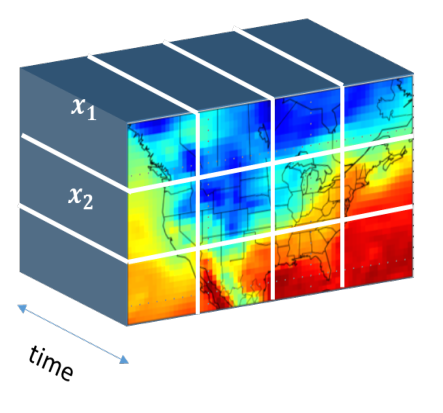
\includegraphics[width=.6\columnwidth]{Figures/data_cube}
  \caption{The cube represents the global variable $h$ in space and
    time. The sub-cubes specified by the white lines are
    $x_i$.}
  \label{fig:data_cube}
\end{figure} 


In \autoref{fig:data_cube}, the global variable $h$ is represented
as a cube. We decompose $h$
into sub-cubes as shown by white lines. Each global variable inside
the sub-cubes corresponds to only one local variable. The global
variables on the border (white lines), however, correspond to more
than one local variable. With 
this definition of $x_i$, the objective
\eqref{eq:l1tf_var_st_mat} decomposes as $\sum_i f_i(x_i)$ where
$f_i(x_i)=-l(y_i\given x_i)+\Lambda_{(i)}^\top |D_{(i)}x_i|$, and
$\Lambda_{(i)}$ and $D_{(i)}$ contain the temporal and spatial
penalties corresponding to $x_i$ only in one sub-cube along with its
boundary. Thus, we now need to use PDIP to solve $N$ problems each of
size $n_i$, which is feasible for small enough
$n_i$. \autoref{alg:conADMM} gives the general version of this
algorithm. A more detailed discussion of this is in Appendix B of the
Supplement where we show how to compute the dual and the derivatives
of the augmented Lagrangian.  

\begin{algorithm}[tb]
  \caption{Consensus ADMM }
  \label{alg:conADMM}
  \begin{algorithmic}[1]
    \STATE {\bfseries Input:} data $y$, penalty matrix $D$, 
    $\epsilon, \rho,\lambda_t,\lambda_s >0$.
    \STATE {\bf Set:} $h\leftarrow 0$, $z\leftarrow 0$, $u\leftarrow
    0$. \COMMENT{Initialization} 
    \REPEAT
    \STATE $\begin{aligned}x_i&\leftarrow\argmin_{x_i} -l(y_i\given
    x_i)+\Lambda_{(i)}^\top |D_{(i)}x_i|\\&\quad+ (u_i)^\top x_i +
    (\rho/2)  \lVert x_i-\tilde{h}_i \rVert_2^2\end{aligned}$. \\\COMMENT{Update local
      vars using PDIP}
    \STATE $h_k\leftarrow (1/S_k)\sum_{\mathscr{G}(i,j)=k} (x_i)_j
    $. \COMMENT{Global update.}
    \STATE $ u_i\leftarrow u_i + \rho (x_i-\tilde{h}_i)$. \COMMENT{Dual update}
    \UNTIL {$\max\left\{\norm{h^{m+1}-h^m},\ \norm{h^m-x^m}\right\} < \epsilon$}
    \STATE {\bf Return:} $h$.
  \end{algorithmic}
\end{algorithm}



Because consensus ADMM breaks the large optimization into
sub-problems that can be solved independently, it is amenable to a
split-gather parallelization strategy via, e.g., the map reduce framework.
In each iteration, the
computation time will be equal to the time to solve each sub-problem
plus the time to communicate the solutions on the master processor
and perform the consensus step. Since each sub-problem is
small, with parallelization, the computation time in each iteration
will be small. In addition, our experiments with several values of
$\lambda_t$ and $\lambda_s$ showed that the algorithm converges in few
hundreds iterations. 
% \attn{Need to redo this:}Solving each sub-problem on a machine with four
% 3.20GHz Intel i5-3470 cores takes less than 3 seconds on average, and
% so for example if we assume that communication time is 10 seconds and
% the algorithm converges in 300 iterations, with parallelization on
% $N_{sub-cubes}$ machines, the algorithm will converge in about 1
% hour. Assuming that we use $N_{sub-cubes}$ machines and that the
% convergence rate of the algorithm is independent of the grid size,
% this time will be independent of the grid size. 
% If we perform these computations on a single machine, the computation
% time grows linearly with $N_{sub-cubes}$. For example, for the data in
% a grid over the united states and using $3\times3\times521$ sub-cubes
% each iteration of the algorithm will take about 20 minutes on a single
% machine and so with 300 iterations it will take several days to
% converge. Given that we need to compute the solution for several
% values of the parameters $\lambda_t$ and $\lambda_s$, this computation
% time is not feasible. 
This algorithm is most useful if we can parallelize the
computation over several machines with low communication cost between
machines. In the next section, we describe 
another algorithm which makes the computation feasible on a single
machine. 

\subsection{Linearized ADMM}
\label{sec:linADMM}

% In this section, we describe \textit{Linearized ADMM algorithm} \cite{parikh_proximal_2014} which, as we will see, makes the computation on a single machine feasible.

Consider the generic optimization problem
$\min_x f(x)+g(Dx)$
where $x\in \mathbb{R}^n$ and $D\in \mathbb{R}^{m\times n}$. Each
iteration of the linearized ADMM
algorithm~\cite{parikh_proximal_2014} for solving this problem 
has the form
\begin{equation}
  \label{eq:linADMM_steps}
  \begin{aligned}
    x & \leftarrow \prox_{\mu f} \left(x - (\mu/\rho)D^\top (D x - z + u )\right)\\
    z & \leftarrow \prox_{\rho g} \left(z + u\right)\\
    u & \leftarrow u + D x - z
  \end{aligned}
\end{equation}
where the algorithm parameters $\mu$ and $\rho$ satisfy $0 < \mu <
\rho/\norm{D}_2^2$, $z,u\in \mathbb{R}^m$ and the proximal operator is
defined as $\prox_{\alpha \varphi}(u) = \min_x \,\, \alpha \cdot
\varphi(x)+\frac{1}{2} \norm{ x-u}_2^2$. Proximal algorithms are feasible
when these proximal operators can be evaluated efficiently which, as
we show next, is the case for our problem.  

%Clearly, \eqref{eq:l1tf_var_st} has this form necessary for using this algorithm.
% The optimization problem 
% form \eqref{eq:linADMM_opt} by defining
% \begin{align}
% & f(x):= \sum_{k} f_k(x_k) := \sum_{k}x_k+y_{k}^2e^{-x_{k}}\\
% & g(z):= \sum_{l} g_l(z_l) := \sum_{l} \lambda_l |z_l|\label{eq:linADMM_fg}\\
% & z = Dx
% \end{align}
% where $y_k$ is the $k^{th}$ entry of the vector whose entries are
% $y_{ijt}$, and $\lambda_l$ is the $l^{th}$ entry of the vector
% $\Lambda^\top=(\lambda_t\textbf{e}_{n_t}^\top|\lambda_s\textbf{e}_{n_s}^\top)$
% (see \autoref{sec:exten}). 
% To perform the steps in \eqref{eq:linADMM_steps}, we need to evaluate
% $\prox_{\mu f}$ and $\prox_{\rho g}$. 
 


\begin{lemma}
  Let $f(x) = \sum_{k} x_{k} + y_{k}^2e^{-x_{k}}$ and $g(x) =
  \norm{x}_1$. Then, 
  \begin{equation}
    \begin{aligned}
      [\prox_{\mu f}(u)]_k &= \mathscr{W}\bigg(\frac{y_k^2}{\mu}
      \exp\bigg(\frac{1-\mu u_k}{\mu}\bigg) \bigg) + \frac{1-\mu u_k}{\mu},\\
      \prox_{\rho g}(u) &= S_{\rho\lambda}(u)
    \end{aligned}
  \end{equation}
  where $\mathscr{W}(\cdot)$ is the \textit{Lambert W function}
  \cite{corless_lambertw_1996},  $[S_{\alpha}(u)]_k = \sign(u_k)(|u_k|
  -\alpha_k)_+$ and $(v)_+=v\vee 0$.
\end{lemma}
% \begin{proof}
%   If $f(x)=\sum_k f_k(x_k)$ then $[\prox_{\mu f}(x)]_k =
%   \prox_{\mu f_k}(u_k)$. So 
%   $[\prox_{\mu f}(u)]_k=\min_{x_k} \,\,
%   \mu\big(x_k+y_{k}^2e^{-x_{k}}\big)+\frac{1}{2}  (x_k-u_k)^2.$
%   Setting the derivative to 0 and solving for $u_k$ gives the
%   result. Similarly, $[\prox_{\rho g}(u)]_\ell=\rho
%   \lambda_\ell |z_\ell|+1/2(z_\ell-u_\ell)^2$. This is not differentiable,
%   but the solution must satisfy $\rho \cdot \lambda_\ell \cdot \partial
%   \big(|z_\ell| \big)=u_\ell-z_\ell$ where $\partial \big(|z_\ell| \big)$ is the
%   sub-differential of $|z_\ell|$. The solution is the soft-thresholding
%   operator $S_{\rho\lambda_\ell}(u_\ell)$.
% \end{proof}

Therefore, \autoref{alg:linADMM} gives a different method for solving
the same problem. For this algorithm, both the primal update and the
soft thresholding step are performed elementwise at each point of the
spatio-temporal grid. It can therefore be extremely fast to perform
these steps. However, because there are now many more dual variables,
this algorithm will require more outer iterations to achieve
consensus. It therefore is highly problem and architecture dependent
whether \autoref{alg:conADMM} or \autoref{alg:linADMM} will be more
useful in any particular context.

\begin{algorithm}[tb]
  \caption{Linearized ADMM }
  \label{alg:linADMM}
  \begin{algorithmic}[1]
    \STATE {\bfseries Input:} data $y$, penalty matrix $D$, 
    $\epsilon, \rho,\lambda_t,\lambda_s >0$.
    \STATE {\bf Set:} $h\leftarrow 0$, $z\leftarrow 0$, $u\leftarrow
    0$. \COMMENT{Initialization} 
    \REPEAT
    \STATE $h_k\leftarrow \mathscr{W}\bigg(\frac{y_k^2}{\mu} 
    \exp\bigg(\frac{1-\mu u_k}{\mu}\bigg) \bigg) + \frac{1-\mu
      u_k}{\mu}$ for all $k=1,\ldots TS$. \COMMENT{Primal update}
    \STATE $z\leftarrow S_{\rho\lambda}(u)$. \COMMENT{Elementwise soft thresholding}
    \STATE $u\leftarrow u + Dh-z$. \COMMENT{Dual update}
    \UNTIL {$\max\{\norm{Dh-z},\; \norm{z^{m+1}-z^m}\} < \epsilon$}
    \STATE {\bf Return:} $z$.
  \end{algorithmic}
\end{algorithm}





\section{Empirical Evaluation}
\label{sec:empirical-evaluation}

In this section, we examine both simulated and real spatio-temporal
climate data. All the computations were performed on a Linux machine
with four 3.20GHz Intel i5-3470 cores. 

\subsection{Simulations}
\label{sec:simulations}

Before examining real data, we apply our model to some synthetic
data. This example was constructed to mimic the types of spatial and
temporal phenomena observable in typical climate data. We generate a
complete spatio temporal field wherein 
observations at all time steps and all locations are
independent Gaussian random variables with zero mean. However, the
variance of these random variables follows a smoothly varying function
in time and space given by the following parametric model:
\begin{align}
  \sigma^2(t,r,c) & =\sum_{k=1}^{K} W_k(t) \cdot \exp\bigg(
                    \frac{(r-r_k)^2+(c-c_k)^2} {2\sigma_k^2} \bigg)\\
  W_k(t) & =\alpha_k \cdot t + \exp(\sin(2\pi\omega_k t+\phi_k)) .
\label{eq:sourceVar}
\end{align}
The variance at each time and location is computed as the
weighted sum of $K$ bell-shaped functions where the weights are
time-varying, consist of a linear trend $\alpha_k \cdot t$ and a
periodic term $\beta_k \cdot \sin(2\pi\omega_k t+\phi_k)$. The
bell-shaped functions impose spatial smoothness while the linear
trend and the periodic terms enforce the temporal smoothness similar
to the seasonal component in the real climate data. We simulated the
data on a 5 by 7 grid and for 780 time steps with $K=4$. This yields a
small enough problem so that it can be evaluated many times while
still mimicking important properties of climate data.
Specific parameter choices of the variance function are shown in
\autoref{tab:sim_params}.
For illustration, we also plot the
variance function for all locations at $t=25$ and $t=45$
(\autoref{fig:true_var_spatial}, top panel) in as well as
the variance across time at $(0,0)$ (bottom panel, orange).
\begin{table}[tb]
  \caption{Parameters used to simulate data.}
  \label{tab:sim_params}
  \begin{center}
    \begin{tabular}{ccccccc}
      \hline
      $s$ & $r_s$ & $c_s$ & $\sigma_s$ &$\alpha_s$ & $\omega_s$ & $\phi_s$\\
      \hline
      1 & 0 & 0 & 5 & 0.5 & 0.121 & 0 \\
      2 & 0 & 5 & 5 & 0.1 & 0.121 & 0 \\
      3 & 3 & 0 & 5 & -0.5 & 0.121 & $\pi/2$ \\
      4 & 3 & 5 & 5 & -0.1 & 0.121 & $\pi/2$ \\
      \hline
    \end{tabular}
  \end{center}
\end{table} 
\begin{figure}[tb]
  \centering	
  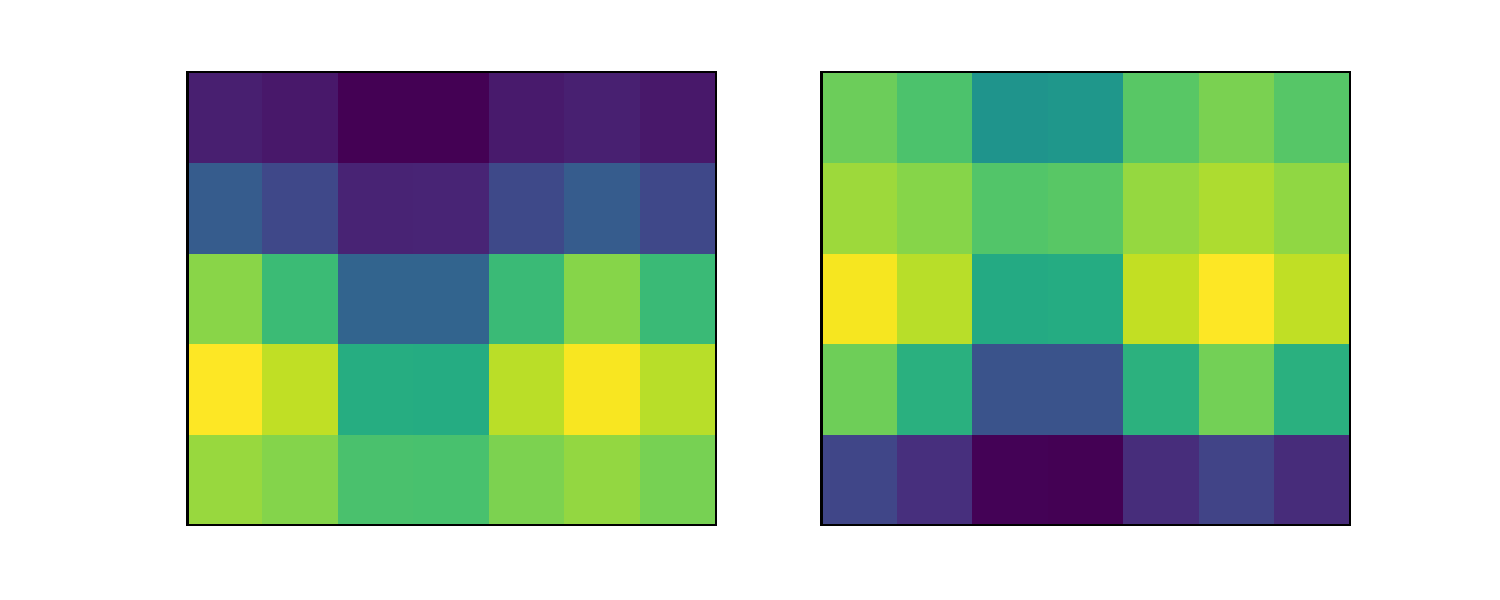
\includegraphics[height=.1\textheight]{Figures/true_var_spatial}\\
  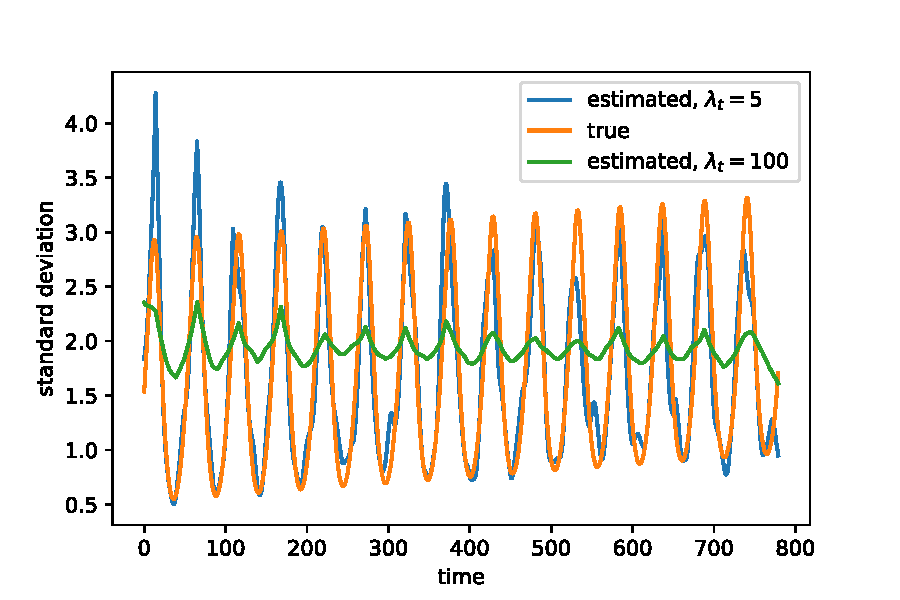
\includegraphics[height=.15\textheight]{Figures/true_fitted_var}
  \caption{Top: Variance function at $t=25$ (left) and $t=45$
    (right). Bottom: The true (orange) and estimated standard deviation 
    function at the location (0,0). The estimated values are
    obtained using linearized ADMM with $\lambda_s=0.1$ and two
    values of $\lambda_t$: $\lambda_t=5$ (blue) and
    $\lambda_t=100$ (green).} \label{fig:true_var_spatial}
\end{figure}




We estimated the linearized ADMM for all combinations of values of
$\lambda_t$ and $\lambda_s$ from the sets $\lambda_t \in
\{0,1,5,10,50,100\}$ and $\lambda_s \in \{0,0.05,0.1,0.2,0.3\}$. For
each pair, we then compute the mean absolute error (MAE) between the
estimated variance and the true variance at all locations and all time
steps. For $\lambda_t=5$ and $\lambda_s=0.1$, the MAE was minimized. 
\begin{figure}[tb]
  \centering	
  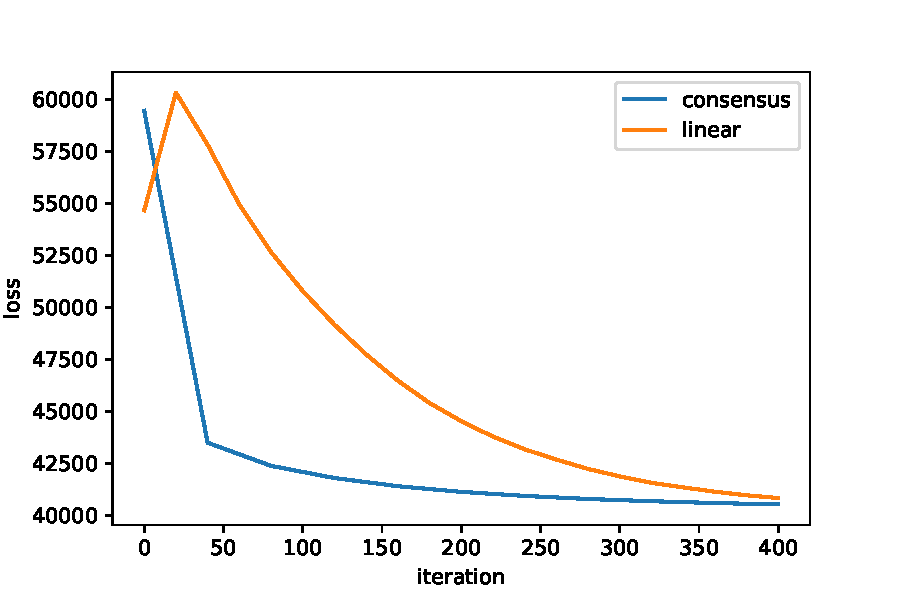
\includegraphics[width=.46\columnwidth]{Figures/convergence}  
  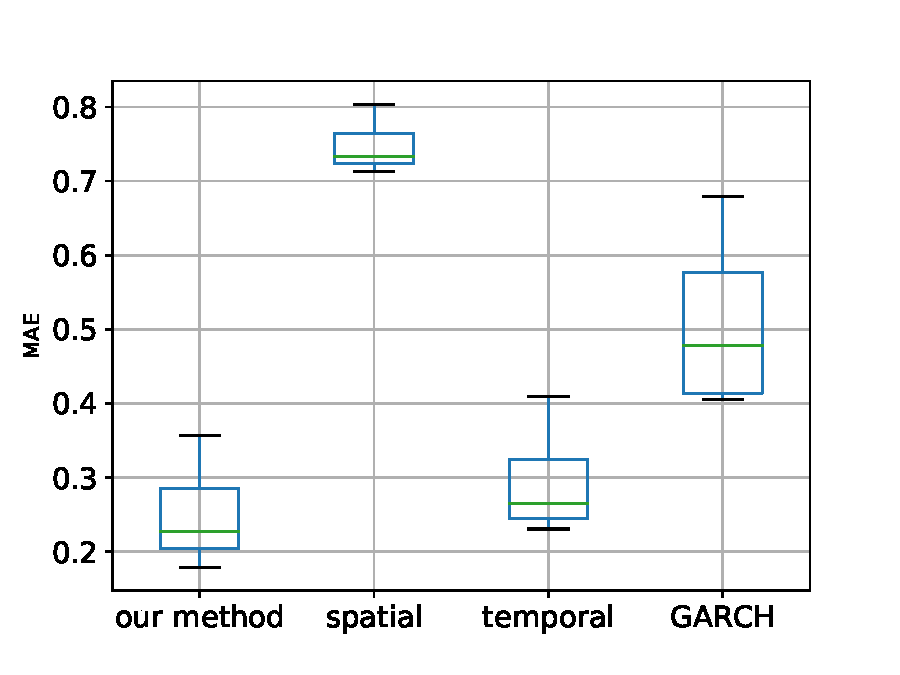
\includegraphics[width=.46\columnwidth]{Figures/modelComp_MAE}  
  \caption{Left: Value of the objective function for linearized (orange)
    and consensus (blue) ADMM against iteration. Right: MAE for (1) our
    method with optimal values of $\lambda_t$ and $\lambda_s$ (2)
    temporal penalty only (3) spatial
    penalty only and (4) a GARCH(1,1).} 
  \label{fig:true_fitted_var}
\end{figure}
The
bottom panel of \autoref{fig:true_var_spatial} shows the true and the
estimated standard deviation at location (0,0) 
and $\lambda_t=5$ (blue) and $\lambda_t=100$ (green) ($\lambda_s=0.1$).
Larger values of $\lambda_t$ lead to estimated values
which are ``too smooth". The left panel of \autoref{fig:true_fitted_var} shows the
convergence of both methods as a function of iteration. It is
important to note that each iteration of the linearized
algorithm takes 0.01 seconds on average while each iteration of the
consensus ADMM takes about 20 seconds. Thus, where the lines meet at
400 iterations requires about 4 seconds for the linearized method and
2 hours for the consensus method.





To further examine the performance of the proposed model, we next
compare it to three alternatives: a model which does not consider the
spatial smoothness (equivalent to fitting the model in
\autoref{sec:l1tf_var} to each time-series separately), a model which only imposes spatial smoothness, and a GARCH(1,1) model. We
simulated 100 datasets using the method explained above with $\sigma_s
\sim \mathsf{uniform}(4,7)$. The right panel of
\autoref{fig:true_fitted_var} shows the boxplot of the MAE for these
models. We note that, using an algorithm akin
to~\citep{HallacPark2017} ignores the spatial component and 

\subsection{Data Analysis}
\label{sec:data}

Consensus ADMM in~\autoref{sec:consOpt} is appropriate when we can
easily parallelize it over multiple machines.  Otherwise, it is significantly
slower, so all the results reported in this section are obtained
using \autoref{alg:linADMM}. We
applied this algorithm to the Northern hemisphere of the ERA-20C
dataset available from the European Center for Medium-Range
Weather Forecasts\footnote{\url{https://www.ecmwf.int}}. We use 
the 2 meter temperature measured daily at 12 p.m from January 1, 1960
to December 24, 2010. 

\paragraph{Preprocessing}

Examination of the time-series alone demonstrates
strong differences 
between trend and cyclic behavior across spatial locations. One might
try to model the cycles by the summation of 
sinusoidal terms with different frequencies. However, for some
time-series this may need many terms to be included in the summation
to achieve a reasonable level of accuracy. In addition, such a model
cannot capture the non-stationarity in the cycles. 

\autoref{fig:cities_ts} shows the time-series of the 
temperature of three cities: Indianapolis (USA), San Diego (USA) and
Manaus (Brazil). The time-series of Indianapolis and San Diego show
clear cyclic behavior, though the amplitude of the cycles
changes. The time-series of Manaus does not
show any regular cyclic behavior. For this reason, we
first apply trend filtering to remove seasonal terms and de-trend
every time series. For each time-series, we found the optimal value of
the penalty parameter using \textit{k-fold cross-validation} with
$k=5$. We used the R package \textbf{genlasso} to perform these
computations \cite{arnold_efficient_2016}.  
\begin{figure}[tb]
	\centering
	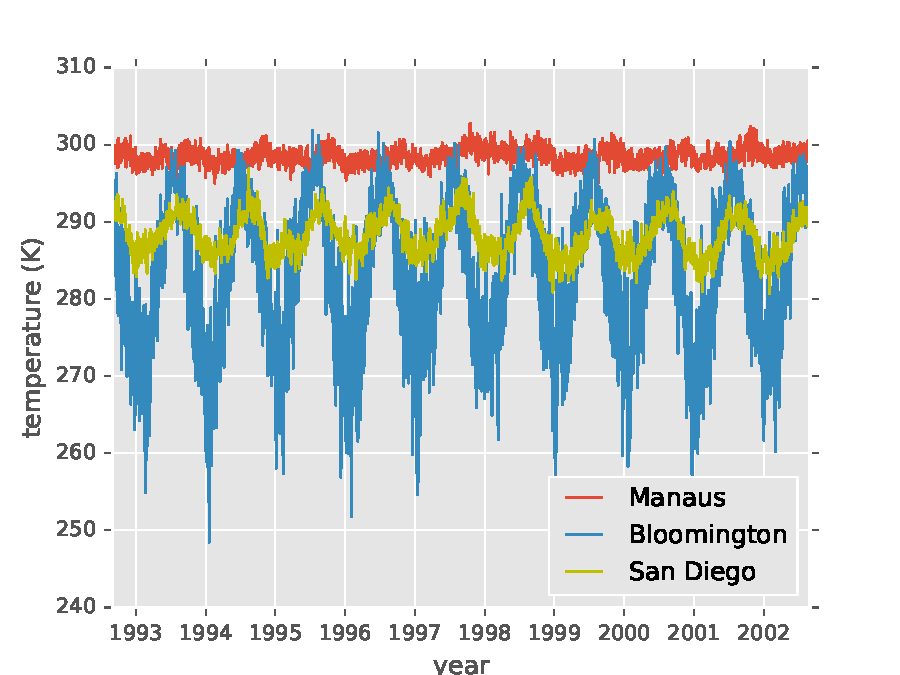
\includegraphics[width=.3\textheight]{Figures/cities_ts}
 	\caption{Time-series of the temperature (in Kelvin) of three cities.}
 	\label{fig:cities_ts}
\end{figure} 
The blue curve in the left panel of Figure
\autoref{fig:bloom_estimatedSD} shows the time-series of the
temperature of Indianapolis after detrending using this method. 


\begin{figure}[tb]
  \centering
  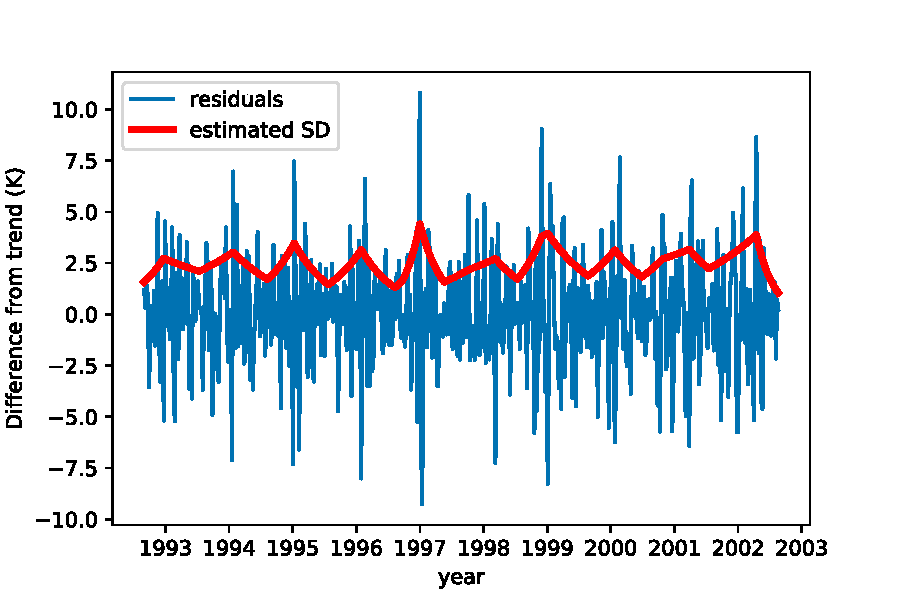
\includegraphics[width=.8 \columnwidth]{Figures/indy_estimatedSD_1}
  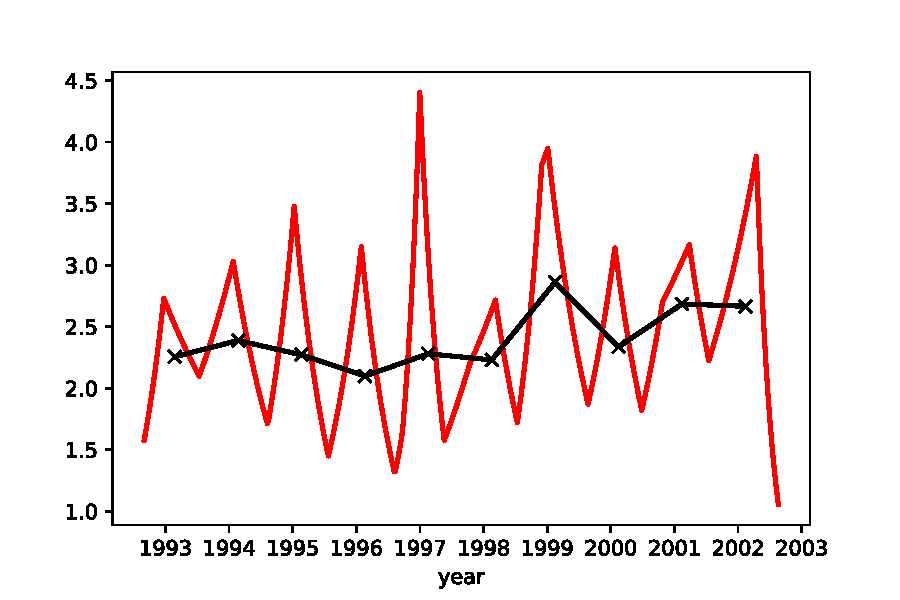
\includegraphics[width=.45 \columnwidth]{Figures/indy_estimatedSD_2}
  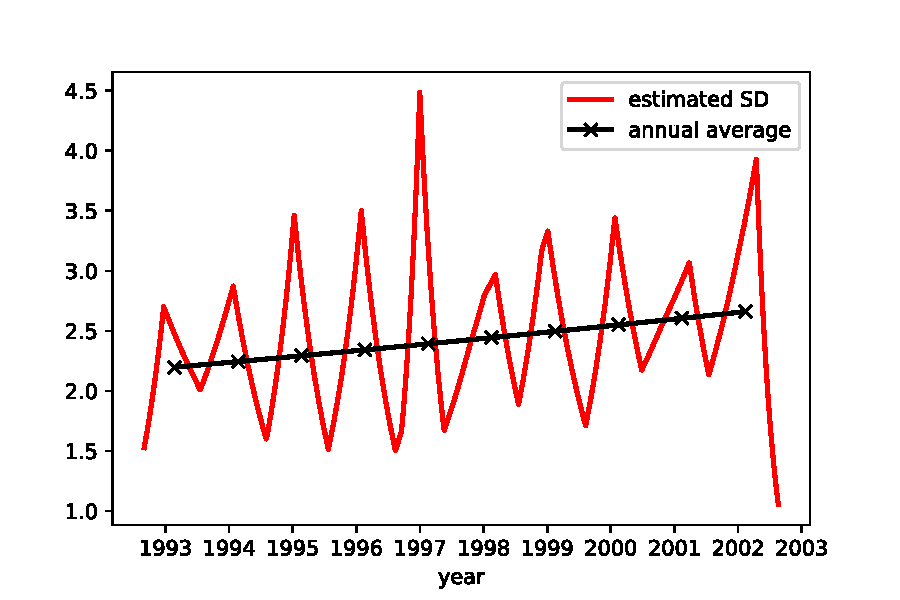
\includegraphics[width=.45 \columnwidth]{Figures/indy_estimatedSD_3}  
  \caption{Left: The residuals of the time-series of Indianapolis
    (averaged weekly) and the estimated SD obtained from the method of
    \autoref{sec:l1tf_var} (red). Middle: the estimated SDs (red) and
    their annual average (black) without imposing the long horizon
    penalty. Right: the same as middle panel but here the long horizon
    penalty is imposed. See the text for more details. \attn{Fix the caption (top-bottom or left right)}} 
  \label{fig:bloom_estimatedSD}
\end{figure} 

The red curve in the left panel of Figure \autoref{fig:bloom_estimatedSD}
shows the estimated SD (which is $\exp(h_t/2)$) of the residuals of
the time-series of Indianapolis obtained from out proposed model. For
ease of analysis, we compute the average
of the estimated SD for each year. Both are shown in the middle panel of
\autoref{fig:bloom_estimatedSD}. To smooth the annual trend, we add
a long horizon penalty to \eqref{eq:l1tf_var}.
The estimated, smoothed SDs are shown
the right panel of \autoref{fig:bloom_estimatedSD}. The annual average
of the estimated SDs shows a linear trend with a positive slope. 

% The Supplement explains some preprocessing and investigates some
% properties of the time-series of different locations on
% earth. \autoref{fig:bloom_estimatedSD} shows a processed time-series for a
% single location.
% The variance of this time-series has an irregular cyclic
% behavior. Additionally, the time-series of other locations show 
% different patterns. These observations motivated the need to develop a
% non-parametric framework for this
% problem. \autoref{fig:bloom_estimatedSD} also shows the
% estimated SD obtained using the method of
% \autoref{sec:l1tf_var}. 


% Since the estimated SD captures the periodic
% behavior of 
% volatility, it is hard to distinguish any long-term trend. Therefore,
% we compute the annual average of these 
% estimates. However, as this figure shows, the annual trend is not
% smooth. This is because in the optimization problem
% \eqref{eq:l1tf_var}, the smoothness of the annual trend is not
% encouraged. Therefore, in Appendix D we propose a simple method to
% encourage the smoothness of the annual average trend. The estimated
% SDs using this method is shown in the right panel of
% \autoref{fig:bloom_estimatedSD}. The annual average of the estimated
% SDs shows a linear trend with a positive slope.  

\paragraph{Convergence}

As shown in \autoref{alg:linADMM}, we evaluated convergence using
$\epsilon=0.001\%$ of the MSE of the data.
Our simulation experiments showed that the
convergence speed depends on the value of $\lambda_t$ and
$\lambda_s$. Furthermore, using the solution obtained for smaller values
of these parameters as a warm start for the larger values, the
converges speed improves.   


\paragraph{Model Selection}
One common method for choosing the penalty parameters in the Lasso
problems is to find the solution for a range of the values of these
parameters and then choose the values which minimize a model selection
criterion. However, such analysis needs the computation of the degrees
of freedom. Several previous work have investigated the df in
generalized lasso problems
\cite{tibshirani_degrees_2012,hu_dual_2015,zeng_geometry_2017}. However,
all these studies have considered the linear regression problem and,
to the best of our knowledge, the problem of computing the df for
generalized lasso with general objective function has not been
considered yet. In this paper, we use a heuristic method for choosing $\lambda_t$ and
$\lambda_s$: we compute the optimal solution for a range of values of
these parameters and choose the values which minimize
$\mathscr{L}(\lambda_t,\lambda_s)=-l(y|h)+ \sum \lVert D_{total}h
\lVert$. This objective is a compromise between the negative log
likelihood ($-l(y|h)$) and the complexity of the solution ($\sum
\lVert D_{total}h \lVert$). For smoother solutions the value of $\sum
\lVert D_{total}h \lVert$ will be smaller but with the cost of larger
$-l(y|h)$. We computed the optimal solution for all the combinations of the
following sets of values: $\lambda_t \in \{0,2,4,8,10,15,200,1000\} \, \, ,
\lambda_s \in \{0,.1,.5,2,5,10\}$. The best combination was
$\lambda_t=4$ and $\lambda_s=2$. All the analyses in the next section
are performed on the solution for these values.  


\paragraph{Analysis of Trends in Temperature Volatility}

\begin{figure}[tb]
  \centering
  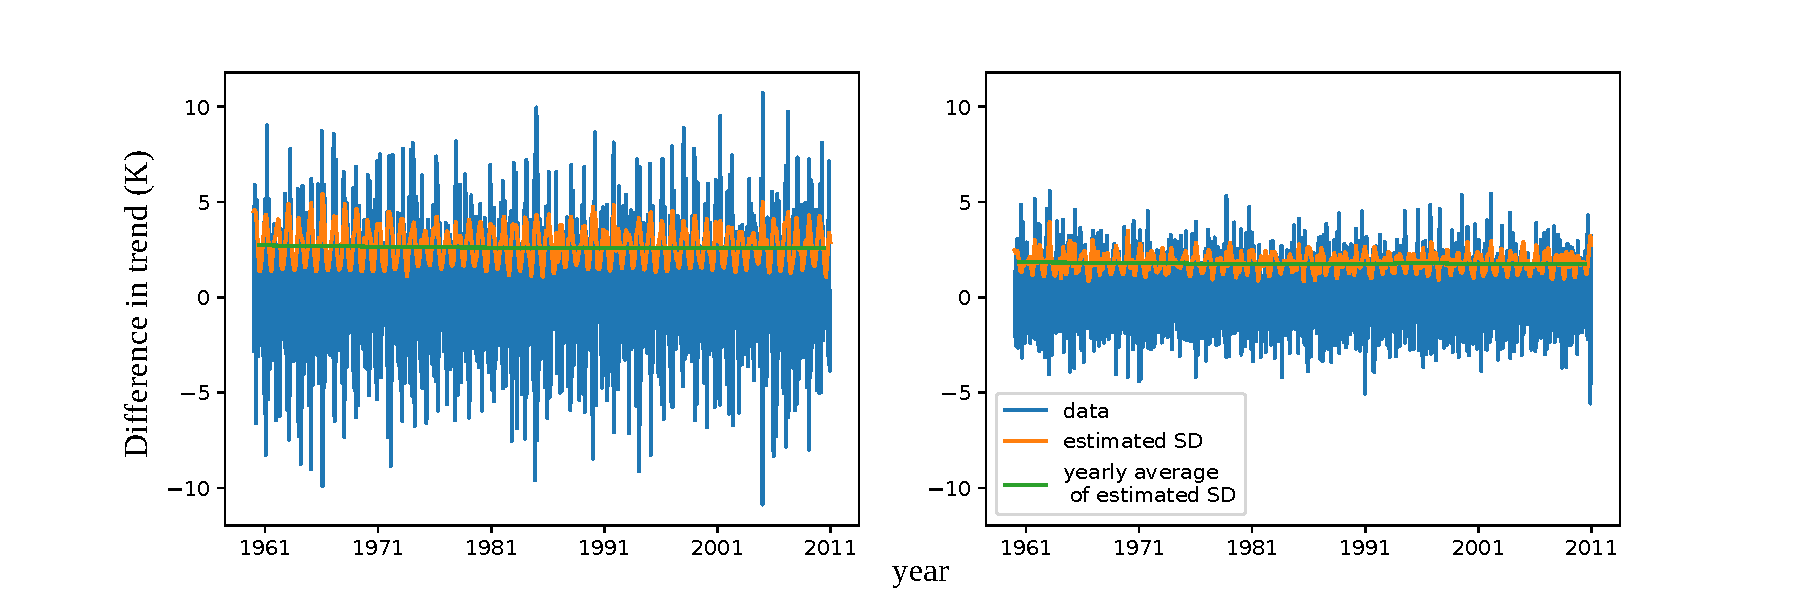
\includegraphics[width=1.1\columnwidth]{Figures/ts_estimatedVar}
  \caption{Detrended data and the estimated SD for
    a small midwestern city (left) and San Diego (right).\attn{Fix these}} 
  \label{fig:avg_change_estimatedSD}
\end{figure} 

The top row of \autoref{fig:avg_change_estimatedSD} shows the
detrended data, the estimated standard deviation and the yearly
average of these estimates for two cities in the US: a small
midwestern city (left) and San Diego (right). The estimated SD
captures the periodic behavior in the variance of the time-series. In
addition, the number of linear segments changes adaptively in each
time window depending on how fast the variance is changing.  
\begin{figure}[tb]
  \centering
  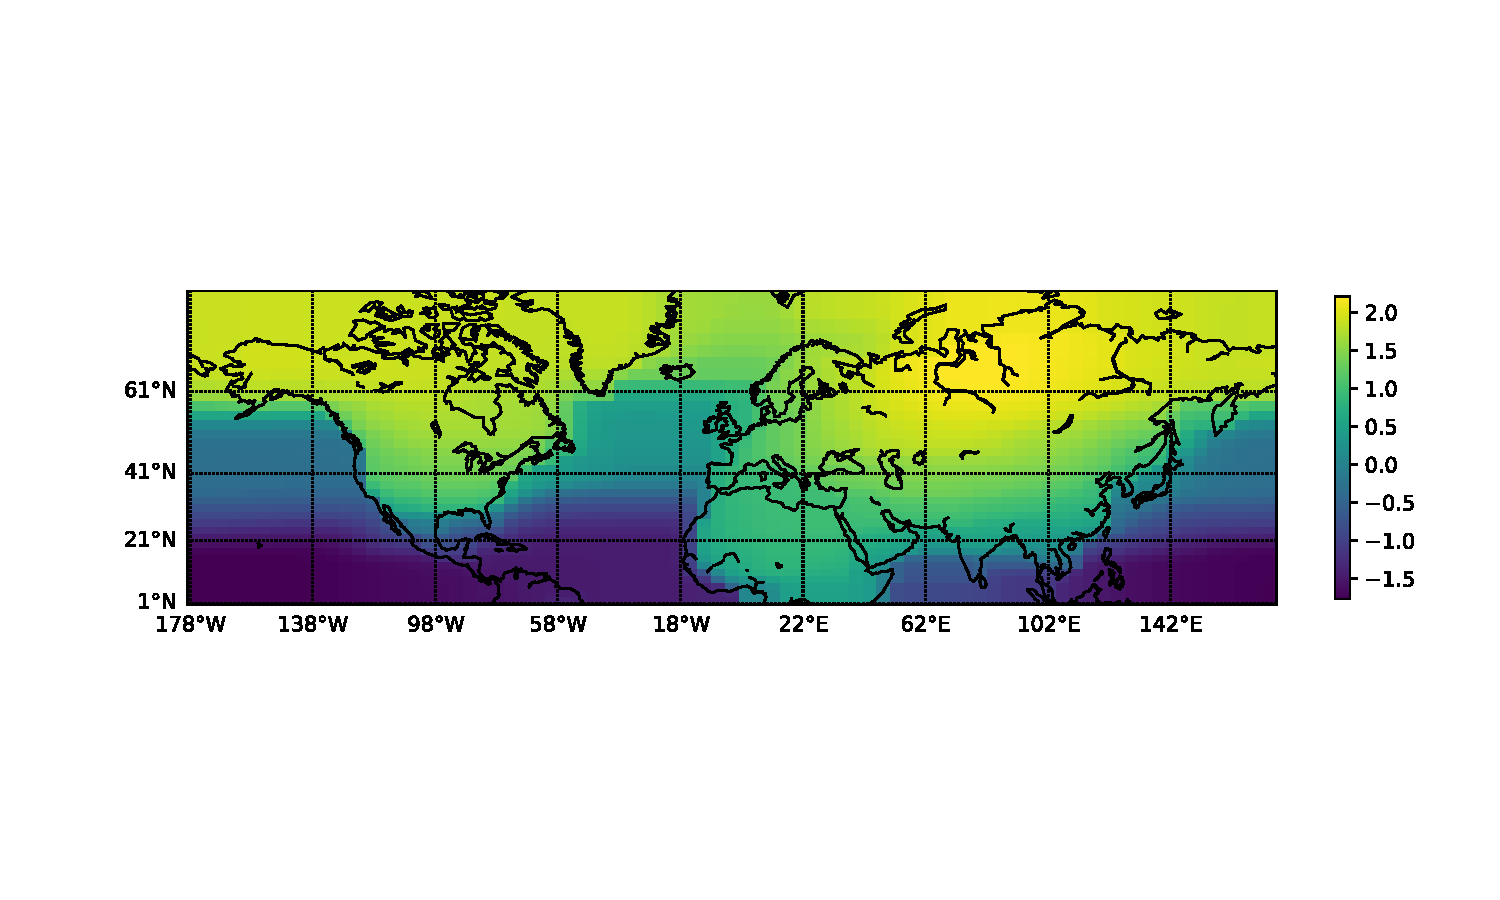
\includegraphics[width=.9\linewidth]{Figures/avg_logVar.pdf}\\
  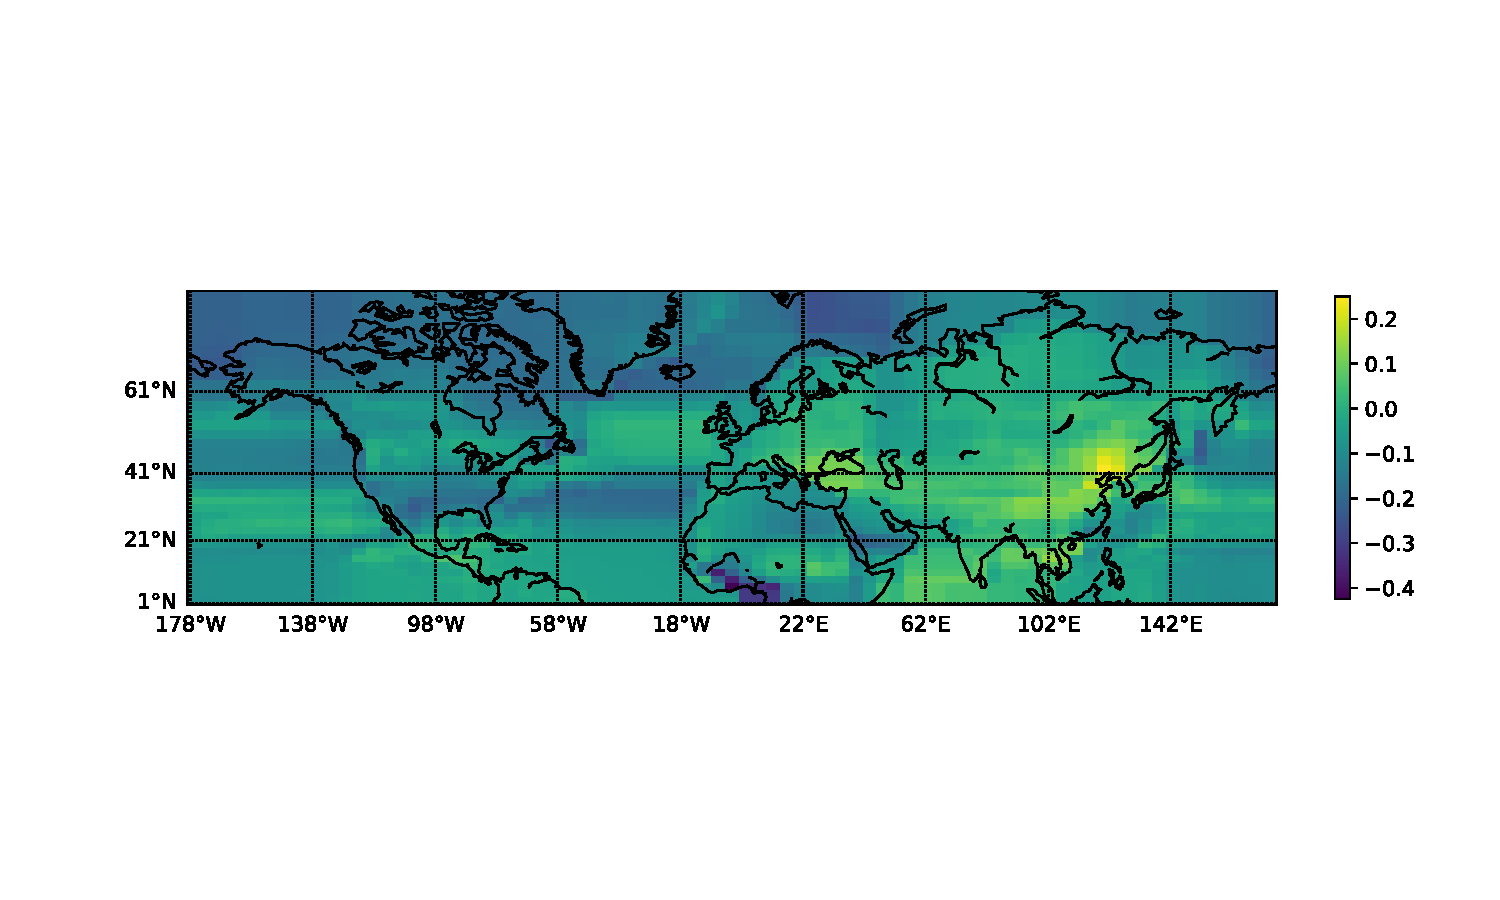
\includegraphics[width=.9\linewidth]{Figures/avg_change_logVar.pdf}
  \caption{The
    average of the detrended estimated variance over the northern hemisphere (top) and the
    change in the variance from 1961 to 2011 (bottom).}
\label{fig:avg_chg}
\end{figure}

The yearly average of the estimated SD captures the trend in the
temperature volatility. For example, we can see that the variance in
the midwestern city displays a small positive trend. To determine how the volatility has
changed in each location, we subtract the average of the estimated
variance in 1961 from the average in the following years and compute
their sum. The value of this change in the variance in each location
is depicted in the right panel of
\autoref{fig:avg_chg}. The left panel of this
shows the average estimated variance in each location. Since the
optimal value of the spatial penalty is rather large ($\lambda_s=2$)
the estimated variance is spatially very smooth. 

The SD in most locations on the northern
hemisphere had a negative trend in this time period, though spatially,
this decreasing pattern is localized mainly toward the extreme
northern latitudes and over oceans. In many ways, this is consistent
with climate change predictions: oceans tend to operate as a local
thermostat, regulating deviations in local temperature, while warming polar
regions display fewer days of extreme cold.
% It is interesting to note that the trend in volatility is almost zero
% over the oceans. 
The most positive trend can be observed in Asia and
particularly in south-east Asia. 

% \begin{figure}[tb]
%   \centering
%   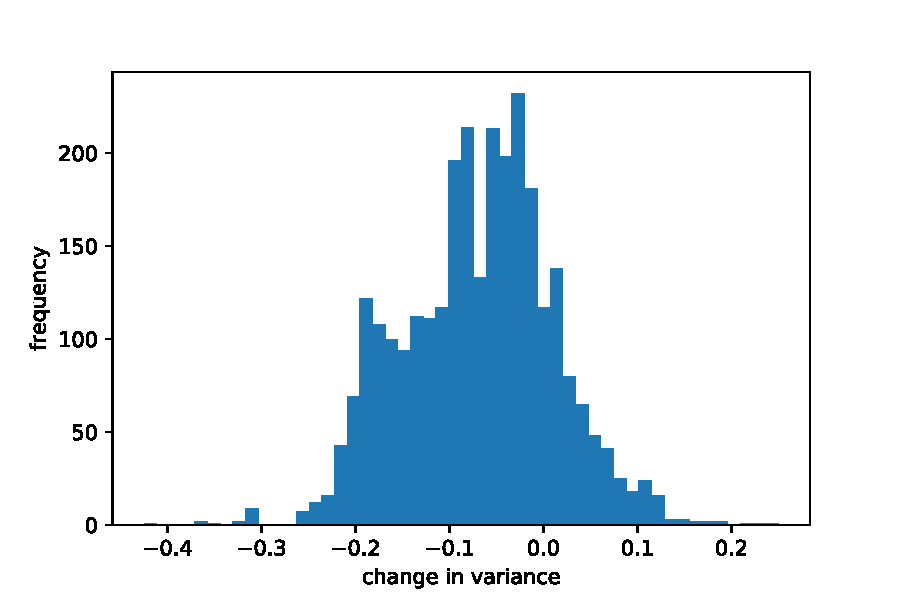
\includegraphics[width=.9\linewidth]{Figures/hist_avg_change.pdf}
%   \caption{The histogram of changes in estimated SD.}
%   \label{fig:hist}
% \end{figure}

% \autoref{fig:hist} shows the
% histogram of change in the estimated SD across the northern
% hemisphere. The SD in most locations on the northern
% hemisphere had a negative trend in this time period, though spatially,
% this decreasing pattern is localized mainly toward the extreme
% northern latitudes and over oceans. In many ways, this is consistent
% with climate change predictions: oceans tend to operate as a local
% thermostat, regulating deviations in local temperature, while warming polar
% regions display fewer days of extreme cold.



 

\section{Discussion}
\label{sec:discussion}

In this paper, we proposed a new method for estimating the variance of
spatio-temporal data. The main idea is to cast this problem as a
constrained optimization problem where the constraints enforce smooth
changes in the variance for neighboring points in time and space. In
particular, the solution is piecewise linear in time and piecewise
constant in space. The resulting optimization is in the form of a
generalized LASSO problem with high-dimension, and so applying the
PDIP method directly is infeasible. We therefore developed two
ADMM-based algorithms to solve this problem: the consensus ADMM and
linearized ADMM. 

The consensus ADMM algorithm converges in a few hundreds of iterations
but each iteration takes much longer than the linearized ADMM
algorithm. The appealing feature of the consensus ADMM algorithm is
that if it is parallelized on enough machines the
computation time per iteration remains constant as the problem size
increases. The linearized ADMM algorithm on the other hand converges
in a few thousand iterations but each iteration is performed in a
split second. However, since the algorithm converges in many
iterations it is not very appropriate for parallelization. The reason
is that after each iteration the solution computed in each machine
should be broadcast to the master machine and this operation takes
some time which depends on the speed of the network connecting the
slave machines to the master. A direction for future research would be
to combine these two algorithms in the following way: the problem
should be split into the sub-problems (as in the consensus ADMM) but
each sub-problem can be solved using linearized ADMM. 

% \attn{We did not do this. Change the below.}
% We applied the linearized ADMM algorithm to the surface temperature
% data on a grid over the united states, for years 1992-2002. The
% results showed that in many locations the variance of the temperature
% has increased about 1 unit in 10 years. 

% The goal of this paper, however, is not to make any conclusions about
% the trend in the variance because we solved the problem only for a
% grid over the united states and for 10 years of the data. A thorough
% analysis, needs the full solution over the globe and for a longer time
% period. The goal of the paper, was to propose the idea of estimating
% the trend in variance of spatio-temporal signals using generalized
% lasso and to investigate the algorithms for solving the resulting
% optimization problem. 

\fontsize{9.0pt}{10.0pt} \selectfont
\bibliographystyle{aaai}
\bibliography{aaai-references}
\clearpage

\appendix
\section{PDIP for $\ell_1$ Trend Filtering of variance}
\label{sec:app_l1tf_var}

In this appendix we provide more details on how to solve the optimization problem with the objective specified in equation \ref{eq:l1tf_var} using PDIP. The objective function is convex but not differentiable. Therefore, to be able to use PDIP we first need to derive the dual of this problem. We note that this is a generalized LASSO problem \citep{TibshiraniTaylor2011}. The dual of a generalized LASSO with the objective $f(x)+\lambda \norm{ Dx }_1$ is:  

\begin{align}
\min_\nu&\quad f^*(-D^\top\nu) & \mbox{s.t.}&\quad \norm{ \nu }_\infty \le \lambda
\end{align}

\noindent where $f^*(\cdot)$ is the Fenchel conjugate of $f$: $f^*(u)=\max_x u^\top x-f(x)$. It is simple to show that for the objective function of Equation \ref{eq:l1tf_var}

\begin{equation}
f^*(u)=\sum_t (u_t-1)\log\frac{y_t^2}{1-u_t} + u_t-1.
\label{eq:conj}
\end{equation}

Each iteration of PDIP involves computing a search direction by taking a Newton step for the system of nonlinear equations $r_w(v,\mu_1,\mu_2)=0$, where $w>0$ is a parameter and

\begin{equation}
  r_w(v,\mu_1,\mu_2):=
	\begin{bmatrix}
	r_{dual}\\
	r_{cent}	
	\end{bmatrix}=
  \begin{bmatrix}
    \nabla f^*(-D^\top v) + \mu_1 - \mu_2\\
    -\mu_1(v-\lambda\one)+\mu_2(v + \lambda\one) -w^{-1}\one
  \end{bmatrix}
\label{eq:resid}
\end{equation}

\noindent for $w>0$, where $\mu_1$ and $\mu_2$ are dual variables for the $\ell_\infty$ constraint. Let $A=[\nabla r_{dual}^\top , \nabla r_{cent}^\top]^\top$. The newton step takes the following form

\begin{equation}
r_w(v,\mu_1,\mu_2)+A
\begin{bmatrix}
	\nabla v\\
	\nabla \mu_1\\
	\nabla \mu_2	
	\end{bmatrix}= 0
\label{eq:newton_step}
\end{equation}


We have:

\begin{equation}
A=
\begin{bmatrix}
	\nabla^2 f^*(-D^\top v) & I & -I\\
	-\mathbf{diag(\mu_1)}\one & -v+\lambda\one & \mathbf{0}\\
	\mathbf{diag(\mu_2)}\one & v+\lambda\one & \mathbf{0}
	\end{bmatrix}
\label{eq:delta_r}
\end{equation}

Therefore, to perform the Newton step we need to compute $\nabla f^*(-D^\top v)$ and $\nabla^2 f^*(-D^\top v)$. It is straightforward to show that

\begin{align}
& \nabla f^*(-D^\top v) =  -\nabla_u f^*(u) D^\top ,\\
& \quad u=-D^\top v, \quad (\nabla_u f^*(u))_j=\log\bigg(\frac{y_j^2}{1-u_j}\bigg) \\
& \nabla^2 f^*(-D^\top v)=D\nabla_u^2 f^*(u)D^\top, \quad (\nabla_u^2 f^*(u))_j=\mathbf{diag}\bigg(\frac{1}{1-u_j}\bigg)
\end{align}


Having computed the conjugate function and its gradient and Jacobian, now we can use a number of convex optimization software packages which have an implementation of PDIP to solve the optimization problem with the objective function \ref{eq:l1tf_var}. We chose the python API of the \texttt{cvxopt} package ~\citep{andersen_cvxopt:_2013}.



\section{PDIP Update in~\autoref{alg:conADMM}}
\label{sec:app_consADMM}

In this section we give more details on performing the $x$-update step in Algorithm 1. We need to solve the following optimization problem:

\begin{equation}
\hat{x}:=\argmin_{x} \bigg( \sum_{j=1}^{n_b} (x_j + y_j^2e^{-x_j}) + (\rho/2) \lVert x-\tilde{z} + u \lVert_2^2 + \Lambda^\top |D x| \bigg)
\label{eq:x_update_opt}
\end{equation}

\noindent where $n_b$ is the number of local variables in each sub-cube in \autoref{fig:data_cube}, and for ease of notation we have dropped the subscript $i$ and superscript $m$. 

The matrix $D$ has the following form:  $D^t=[D_{temp}^t|D_{spat}^t]$. The matrix $D_{temp}$ is the following block-diagonal matrix and corresponds to the temporal penalty: 
\begin{equation}
D_{temp}=\begin{bmatrix}
D_t &  & \\ 
& \ddots & \\
&  & D_t
\end{bmatrix}
\label{eq:d_t_matrix}
\end{equation}

\noindent where $D_t$ was first introduced in Section 2 of the main text and has the following form:

\begin{equation}
 D_t=\begin{bmatrix}
 1 & -2 & 1 &  &  &  &\\ 
 & 1 & -2 & 1 &  &  &\\ 
 &  & \ddots & \ddots & \ddots  &  &\\ 
 &  & & 1 & -2 & 1 &  \\ 
 &  &  &   & 1 & -2 & 1 
 \end{bmatrix}
\label{eq:d_matrix}
\end{equation}

The number of the diagonal blocks in $D_{temp}$ is equal to the grid size $n_r \times n_c$. Each row of the matrix $D_{spat}$ corresponds to one spatial constraint in Equation \eqref{eq:l1tf_var_st} in the text. For example, the first $T$ rows correspond to $|h_{11t}-h_{21t}|$ for $t=1,...,T$, the next $T$ rows correspond to $|h_{11t}-h_{12t}|$, and so on. 


This optimization problem, is again a generalized LASSO problem with $f(x)=\sum_{j=1}^{n_b} (x_j + y_j^2e^{-x_j}) + (\rho/2) \lVert x-\tilde{z} + u \lVert_2^2$. 

As it was explained in Appendix A, the dual of this optimization problem is: $\min_\nu f^*(-D^\top\nu)$ with the constraints $|\nu_k| \le \Lambda_k$. To use PDIP we first need to compute the conjugate function $f^*(\cdot)$. We have:


\begin{align}
f^*(\xi) & = \max_x \quad \xi^\top x - f(x)\\
& =  \max_x \quad \sum_{j=1}^{n_b} (\xi_jx_j - x_j - y_j^2e^{-x_j} - (\rho/2)(x_j-\tilde{z}_j+u_j))
\label{eq:conjugate}
\end{align}

Setting the derivative of the terms inside the summation to 0, we obtain:

\begin{equation}
\xi_j-y_j^2e^{-x_j^*}-\rho x_j^* + \rho (\tilde{z}_j-u_j)=0
\label{eq:x_start}
\end{equation}

\noindent where $x^*$ is the maximizer in \ref{eq:conjugate}. Then, it can be shown that $x_j^*$ which satisfies \eqref{eq:x_start} can be obtained as follows:

\begin{align}
x^*_j & = \mathscr{W}\bigg(\frac{y_j^2}{\rho} e^{\phi_j} \bigg) - \phi_j \\
\phi_j & =\frac{1-\xi_j-\rho(\tilde{z}_j-u_j)}{\rho}
\end{align}

In this equation, $\mathscr{W}(\cdot)$ is the \textit{Lambert function} \cite{corless_lambertw_1996}. Finally, the conjugate function is: $f^*(\xi) = \sum_{j=1}^{n_b} (\xi_jx^*_j - x^*_j - y_j^2e^{-x^*_j} - (\rho/2)(x^*_j-\tilde{z}_j+u_j))$.

To use PDIP, we also need to evaluate $\nabla f^*$ and $\nabla^2 f^*$. First note that $\frac{\partial \mathscr{W}(q)}{\partial q} = \frac{\mathscr{W}(q)}{q(1+\mathscr{W}(q))}$ and $\frac{\partial^2 \mathscr{W}(q)}{\partial q^2} = - \frac{\mathscr{W}^2(q)(\mathscr{W}(q)+q)}{q^2(1+\mathscr{W}(q))^3}$. Using the chain rule we get:

%\x^*_j + \xi_j + \frac{\partial \x^*_j}{\partial \xi_j}

\begin{equation}
\frac{\partial f^*(\xi)}{\partial \xi_j}  =  x^*_j  + \frac{\partial x^*_j}{\partial \xi_j} \bigg[ \xi_j -1 + y_j^2 e^{-x_j^*} + \rho (\tilde{z}_j - u_j - x_j^*) \bigg]
\label{eq:d_f*_start}
\end{equation}
where we have:

\begin{equation}
\frac{\partial x_j^*}{\partial \xi_j}  = \frac{1}{\rho(1+\mathscr{W}((y_j^2/\rho) e^{-\phi_j} ))}
\label{eq:d_x*_start}
\end{equation}

By some tedious but straightforward computation we can obtain the second derivatives:


\begin{align}
\frac{\partial^2 f^*(\xi)}{\partial \xi_j^2} & =  \frac{\partial x_j^*}{\partial \xi_j} - \rho \frac{\partial^2 x_j^*}{\partial \xi_j^2} \bigg[ \phi_j +x_j^* - \tilde{z}_j + u_j \bigg]\\
& \quad + \frac{\partial x_j^*}{\partial \xi_j} \bigg[ 1-y_j^2 \frac{\partial x_j^*}{\partial \xi_j} e^{-x_j^*} -\rho \frac{\partial x_j^*}{\partial \xi_j} \bigg]
\label{eq:d2_f*_start}
\end{align}


\begin{equation}
\frac{\partial^2 x_j^*}{\partial \xi_j^2}  = \frac{\mathscr{W}((y_j^2/\rho) e^{-\phi_j} )}{\rho^2(1+\mathscr{W}((y_j^2/\rho) e^{-\phi_j} ))^3}
\label{eq:d2_x*_start}
\end{equation}

 

% \section{Appendix C}
% \autoref{tab:sim_params} lists the parameters used for simulating data
% in \autoref{sec:simulations}. \autoref{fig:true_var_spatial} shows the
% variance function obtained from there parameters at $t=25$ (left) and
% $t=45$ (center). 

% \begin{table}[tb]
%   \caption{Parameters used to simulate data.}
%   \label{tab:sim_params}
%   \begin{center}
%     \begin{tabular}{ccccccc}
%       \hline
%       $s$ & $r_s$ & $c_s$ & $\sigma_s$ &$\alpha_s$ & $\omega_s$ & $\phi_s$\\
%       \hline
%       1 & 0 & 0 & 5 & 0.5 & 0.121 & 0 \\
%       2 & 0 & 5 & 5 & 0.1 & 0.121 & 0 \\
%       3 & 3 & 0 & 5 & -0.5 & 0.121 & $\pi/2$ \\
%       4 & 3 & 5 & 5 & -0.1 & 0.121 & $\pi/2$ \\
%       \hline
%     \end{tabular}
%   \end{center}
% \end{table} 

% \begin{figure}[tb]
%   \centering	
%   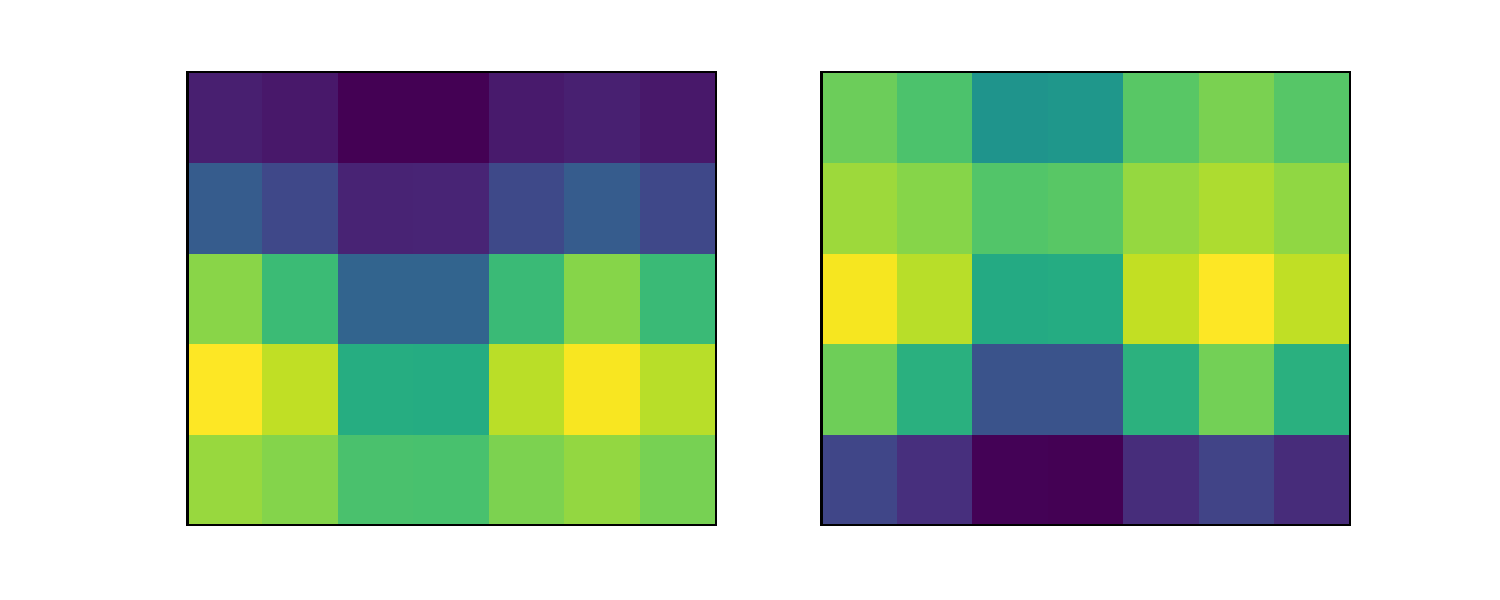
\includegraphics[height=.15\textheight]{Figures/true_var_spatial}
%   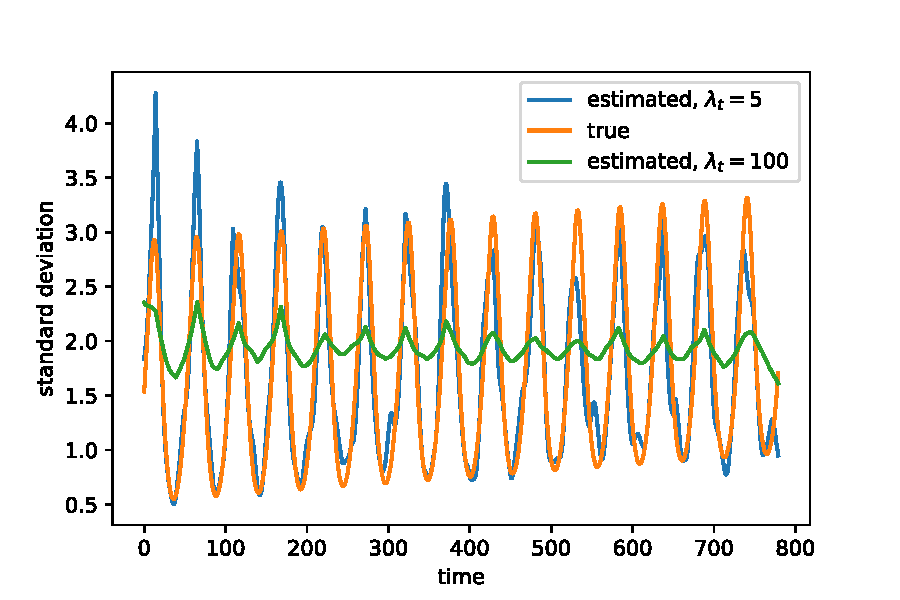
\includegraphics[height=.15\textheight]{Figures/true_fitted_var}
%   \caption{Variance function at $t=25$ (left) and $t=45$
%     (center). Right: the true (orange) and estimated standard deviation 
%     function at the location (0,0). The estimated values are
%     obtained using linearized ADMM with $\lambda_s=0.1$ and two
%     values of $\lambda_t$: $\lambda_t=5$ (blue) and
%     $\lambda_t=100$ (green).} \label{fig:true_var_spatial}
% \end{figure}

\section{Data Exploration}

In this appendix we examine some of the properties of the time-series
of the temperature in ERA-20C dataset. The goal here is to demonstrate
some of the difficulties in modeling the trend in the temperature
volatility and motivate our methodology. 

Figure \autoref{fig:cities_ts} shows the time-series of the
temperature of three cities: Indianapolis (USA), San Diego (USA) and
Manaus (Brazil). The time-series of Indianapolis and San Diego show
clear cyclic behavior. However, while it seems (qualitatively) that
these cycles can be modeled by a sinusoidal function for Indianapolis,
the same is not true for San Diego. Also, the amplitude of the cycles
changes from some years to others. The time-series of Manaus does not
show any regular cyclic behavior. This demonstrates the first
difficulty in analyzing the variance of this data: to analyze the
variance, we first need to remove the cyclic terms from all
time-series. However, there is a lot of variations in the cyclic
behavior of the time-series of different locations. In addition, some
of these cycles cannot be easily modeled by a parametric function
\footnote{One might try to model the cycles by the summation of
  sinusoidal terms with different frequencies. However, for some
  time-series this may need many terms to be included in the summation
  to achieve a reasonable level of accuracy. In addition, this model
  cannot capture the non-stationarity in the cycles.}. To overcome
these issues, we use a non-parametric approach to remove the cyclic
terms from the time-series and de-trend them. This approach, called
\textit{$\ell_1$-trend filtering} is explained in Section 2 of the
text. We detrended each time-series separately using this method. For
each time-series, we found the optimal value of the penalty parameter
using \textit{k-fold cross-validation} with $k=5$. We used the R
package \textbf{genlasso} to perform these computations
\cite{arnold_efficient_2016}.  


\begin{figure}[tb]
	\centering
	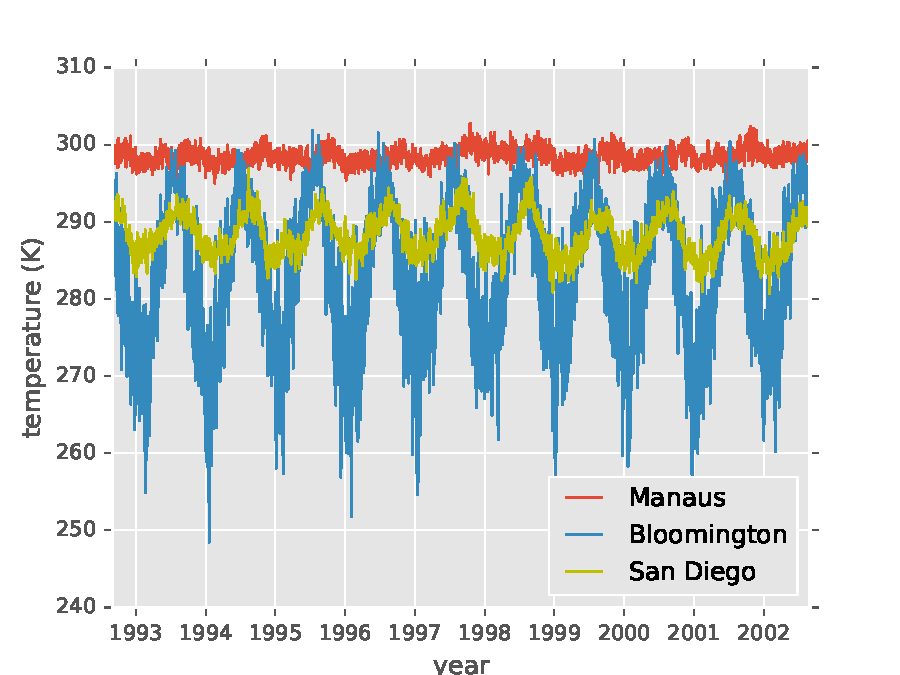
\includegraphics[width=.2\textheight]{Figures/cities_ts}
 	\caption{Time-series of the temperature (in Kelvin) of three cities.}
 	\label{fig:cities_ts}
\end{figure} 

The blue curve in the left panel of Figure \autoref{fig:bloom_estimatedSD} shows the time-series of the temperature of Indianapolis after detrending using this method. This figure, reveals another difficulty in estimating the trend of volatility in this data: the variance of this signal, shows cyclic behavior. Also, the cycles are not regular and their amplitude and frequency change. Even if one can describe the behavior of the variance of the time-series at all locations using a single parametric model (for example a variant of the GARCH models \citep{bollerslev_generalized_1986}), it is not clear how the trend in the variance should be investigated in this framework. These observations motivate the need to develop a non-parametric framework for the problem at hand.

\begin{figure}[tb]
  \centering
  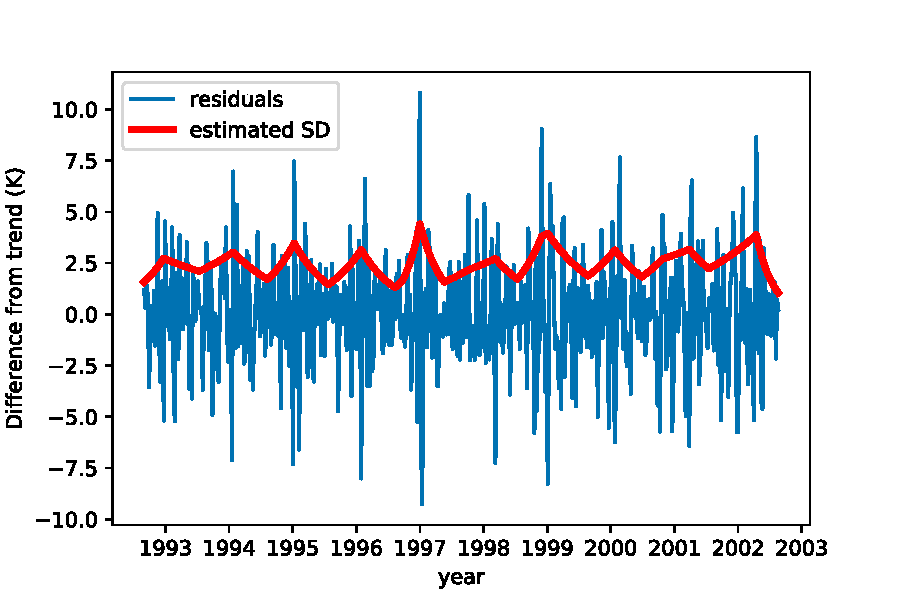
\includegraphics[width=\columnwidth]{Figures/indy_estimatedSD_1}
  \caption{Left: The residuals of the time-series of Indianapolis
    (averaged weekly) and the estimated SD obtained from the method of
    \autoref{sec:l1tf_var} (red). Middle: the estimated SDs (red) and
    their annual average (black) without imposing the long horizon
    penalty. Right: the same as middle panel but here the long horizon
    penalty is imposed. See the text for more details.} 
  \label{fig:bloom_estimatedSD}
\end{figure} 


The red curve in the left panel of Figure \autoref{fig:bloom_estimatedSD}
shows the estimated SD (which is $\exp(h_t/2)$) of the residuals of
the time-series of Indianapolis obtained from out proposed model. To reduce the number of time-steps we work on the weekly averaged of the data. The curve of the estimated SD captures the periodic variations in the
SD of the signal. Just by looking at this curve, it is hard to say if
the SD is decreasing or increasing. Therefore, we compute the average
of the estimated SD for each year. The estimated SD together with this
annual average is shown in the middle panel of
\autoref{fig:bloom_estimatedSD}. As it can be seen, the annual trend
is not smooth. This is because in the optimization problem
\eqref{eq:l1tf_var}, the smoothness of the annual trend is not
encouraged. To remedy this, we add the following long horizon penalty to \eqref{eq:l1tf_var}:
 
\begin{equation}
\sum_{i=1}^{N_{year}-2} \Big\arrowvert \sum_{t=1}^{52} h_{t_1}-2h_{t_2}+h_{t_3}  \Big\arrowvert
\label{eq:lh_penalty}
\end{equation}

where $t_1=52(i-1)+t$, $t_2=52i+t$ and $t_3=52(i+1)+t$. Also,
$N_{year}$ is the number of years over which we are performing our
analysis (here $N_{year}=10$). Since we are working on the weekly
averaged data, each year corresponds to 52 observations. In the matrix
form, the penalty \eqref{eq:lh_penalty} adds $N_{year}$ rows to the
matrix $D$. The estimated SDs using this penalty matrix is shown in
the right panel of \autoref{fig:bloom_estimatedSD}. The annual average
of the estimated SDs shows a linear trend with a positive slope. 



\end{document} 

